\documentclass[american]{ntnuthesis}

\title{Gaussian Processes for long-term trajectory prediction using historical AIS data }
\shorttitle{Gaussian Process AIS Trajectory Prediction}
\author{%
Håvard Skåra Mellbye
\vspace{1cm}\\
Supervisor: Edmund Førland Brekke \\ 
Co-supervisor: Trym Tengesdal
}
\shortauthor{Mellbye}
\date{}


\addbibresource{thesis.bib}

\usepackage{tikz}
\usetikzlibrary{bayesnet}
\usepackage{ifthen}
\usepackage[many]{tcolorbox}
\usepackage{todonotes}
\definecolor{bleu-de-france}{cmyk}{0.79, 0.39, 0.00, 0.09}
\definecolor{bleu-de-france-light}{cmyk}{0.11, 0.04, 0.00, 0.01}




% From https://www.overleaf.com/learn/latex/Glossaries

\makeglossaries % Prepare for adding glossary entries



% --------------------
% ----- Acronyms -----
% --------------------

\newacronym{gp}{GP}{Gaussian Process}
\newacronym{mcmc}{MCMC}{Markov Chain Monte Carlo}
\newacronym{pgm}{PGM}{Probabilistic Graphical Model}
\newacronym{bp}{BP}{Belief Propagation}
\newacronym{dgm}{DGM}{Directed Graphical Model}
\newacronym{bn}{BN}{Bayesian Network}
\newacronym{mrf}{MRF}{Markov Random Field}
\newacronym{kl}{KL}{Kullback-Liebler divergence}
\newacronym{pdf}{PDF}{Probability Density Function}
\newacronym{pmf}{PMF}{Probability Mass Function}
\newacronym{vi}{VI}{Variational Inference}
\newacronym{elbo}{ELBO}{Evidence Lower Bound}
\newacronym{hmc}{HMC}{Hamiltonian Monte Carlo}
\newacronym{nuts}{NUTS}{No-U-Turn sampler}
\newacronym{colav}{COLAV}{Collision Avoidance}
\newacronym{ml}{ML}{Machine Learning}
\newacronym{sog}{SOG}{Speed Over Ground}
\newacronym{cog}{COG}{Course Over Ground}
\newacronym{rbf}{RBF}{Radial Basis Function}

\newglossaryentry{moralization}
{
    name=moralization,
    description={The process of converting Directed Graphical Models into Markov Random Fields}
}

\newglossaryentry{support}{
    name=support,
    description={The set of possible outcomes/values with a non-zero probability, i.e. all events that can happen. A Gaussian distribution for example have support for $x \in \mathcal{R}$ since it has a non-zero probability, $p(x) > 0$, for all real numbers $x \in \mathcal{R}$.}
}

\newglossaryentry{colregs}{
    name=COLREGS,
    description={International Regulations for Preventing Collisions at Sea, a set of rules for ships navigating at sea.}
} % add glossary and acronym lists before document

\begin{document}
\tcbset{colback=bleu-de-france-light, colframe=bleu-de-france}
% gives the width of the current document in pts
\chapter*{Preface}

I want to thank my supervisors Edmund Førland Brekke and Trym Tengesdal for all your guidance and especially for allowing me the freedom to focus on the topics I find the most interesting. As a result, I have had the opportunity to dive deep into the world of probabilistic methods and Bayesian Inference. I also want to thank Ravinder Praveen Kumar Jain for your openness and your insight into long-term trajectory prediction.

I want to thank my family for all your support throughout my studies and growing up. The math homework I had to do as a child did pay off eventually. My grandmother, Anne-Marie Mellbye, has also given me tons of support, and I will be forever grateful!   

My partner in crime, Kristine Stray, deserves a tremendous amount of credit. You have patiently listened to me blabbering about statistics and probability theory, and even though I know you are not as amazed as me, you still encourage me to continue! So for this thesis, I especially want to thank you both for helping me keep motivated as well as giving me valuable input. 


This work marks the end of my graduate studies in Cybernetics and Robotics Engineering at the Norwegian University of Science and Technology. I want to dedicate this thesis to my grandfather, Hans Jørgen Mellbye, who graduated from NTH in 1963 as an electrical engineer. He introduced me to the amazing world of engineering at an early age, which has become a crucial part of who I am today. 


\chapter*{Abstract}

Autonomous ships depend on situational awareness in order to avoid collisions in a safe and robust manner. By knowing the intention of surrounding vessels, safety margins can be improved by avoiding situations with increased risk. In this thesis, methods for Bayesian Inference will be explored, with the goal of developing a flexible framework for intention modelling. Exact and approximate inference methods are explored. Approximate methods are found to be more flexible, allowing easier incorporation of existing knowledge from domain experts or conventions such as \Gls{colregs}. Methods such as \acrfull{mcmc} and \acrfull{vi} are therefore explored further and compared on an illustrative intention model. The results then find \acrshort{mcmc} to be accurate at the cost of computational complexity. \acrshort{vi} on the other hand, is found to be a lot faster, though much less precise on the illustrative model. 
\chapter*{Sammendrag}



\tableofcontents
\listoffigures
\listoftables
%\lstlistoflistings


\printglossary[type=\acronymtype] % Print acronyms
\printglossary                    % Print glossary

\chapter{Introduction}

Humans, while resourceful, are prone to loss of focus, tiredness and have limited attention span. Human errors are estimated to contribute to more than $75\%$ of maritime accidents \cite{Tengesdal2020RiskbasedAM}. On the contrary, computers always remain "focused" and never gets tired. Using autonomus ships in order to reduce the potential for human errors can greatly reduce the number of maritime accidents.
While completely avoiding humans at sea would increase safety, it simply is unrealistic. Autonomous ships will need cooperate with humans on nearby vessels to avoid dangerous situations. Such up-to-date situational awareness is critical to develop decision-making systems in dynamic environments \cite{endsley}. Robust \acrfull{colav} are necessary to  maneuver in areas with potential obstacles in order to avoid collisions. However, the optimal decision is usually highly situation-dependent and requires ability to understand and predict the traffic patterns of nearby vessels, either controlled by humans or autonomous. The optimal decision are further influenced by conventions such as \Gls{colregs}, especially for larger vessels. Still, some scenarios may even require rules and conventions to be broken due to unforeseen circumstances.
However, teaching machines situational awareness is not an easy task. Human's remarkable ability to recognize situations from observations is very hard to replicate in an autonomous systems.

\section{Existing research}
 Existing research on intention modelling for autonomous ships is limited. \cite{Tengesdal2020RiskbasedAM} propose a Probabilistic Scenario-Based Model Predictive Control scheme which is able to utilize probabilistic information about obstacle intentions. It demonstrates how it is possible to make safer decisions when utilizing the additional intent information. The paper propose a general framework for intention inference using \acrfull{bn}, allowing several factors to influence an obstacle's intention. However, the paper only propose an illustrative model where the parameters of the model are assumed known and do not further discuss how these models can be found or used in practice.  

Some related research has been made in the area of autonomous cars. \cite{song} explore how Hidden Markov Models (HMM) can be used to infer the intention of cars in an intersection and then utilize this information in a partially observable Markov decision process (POMDP). 


\section{Bayesian Networks}
Bayesian Networks, often called Belief Networks, are Probabilistic Graphical Models represented as directed acyclic graphs \cite{murphy}. There is strictly speaking nothing Bayesian about Bayesian Networks (they may just as well be used with Frequentist statistics), as it is simply a way to describe probability distributions. Bayesian Networks are also often used to represent causal relations, though the interactions are in no way required to be causal. However, the causal interpretation of Bayesian Networks allow humans to intuitively understand relations between variables. Bayesian Networks are for this reason heavily used in Causal Inference, which attempts to model and infer true causal relationships between variables \cite{causal}. Bayesian Networks intuitive structure further allows human domain experts to reason about and participate in the development of statistical models, without requiring deep statistical knowledge. 
This makes Bayesian Networks a good choice for intention models, as the model need to incorporate prior knowledge such as intuitive reasoning, human experts and predefined rules (such as \Gls{colregs}), as well as be able to learn from new and historical observations. 

\section{Goal}
This thesis will investigate how inference can be performed from available data in a Bayesian Network. At this point the goal is not to find a realistic intention model, but rather try to develop a flexible framework for inference in a known model. Methods which makes few assumptions about the model and makes it easy to incorporate existing knowledge will be the main focus of this thesis. This choice comes from a belief that a good intention model will need to strongly rely on prior knowledge from human experts and from predefined rules. Restricting the model by assumptions made by the inference methods, may end up restricting the ability to accurately encode such information into the model. Approximate Methods such as \acrfull{mcmc} and \acrfull{vi} will therefore be explored in greater detail, while exact methods are only presented as possible solutions for special cases where the assumptions are reasonable. The methods can in some cases be combined, by utilizing exact inference wherever the assumptions are reasonable, and fall back to approximate methods on the parts where exact methods falls short \cite{winnbishop}.
This thesis is structured into multiple chapters. Some necessary theoretical background, mainly an introduction to Bayesian Statistics and \acrfull{pgm}'s, are presented in \cref{chap:theory}. The theory for \acrshort{mcmc} based methods are then found in \cref{chap:mcmc}, while exact and approximate analytical methods are found in \cref{chap:analytical}. In order to not only present the theoretical concepts, implementations of \acrshort{mcmc} and \acrshort{vi} are compared on a fictitious model in \cref{chap:impl}. Finally, the theory and results for the different methods are then compared and discussed in \cref{chap:discussion}.
\chapter{Previous Work}\label{chap:prior_work}

There is currently limited work available on using \acrshort{gp}s on \acrshort{ais} data.

\citeauthor{gpanomaly} propose a method for anomaly detection of moving vessels in \cite{gpanomaly}. The approach uses a \acrshort{gp} to learn vessels' normal behavior in an area, which is then used to detect abnormal behavior. The work further addresses the computational challenges when using large datasets and proposes an active learning approach that iteratively adds new training samples to select the optimal training sample. A relatively small sample size is then used to represent the entire dataset. Active learning is computationally feasible by updating the Cholesky decomposition at each step instead of recomputing the entire decomposition. While the approach works well for anomaly detection, it was not intended for predicting future trajectories, only to classify existing trajectories.

\citeauthor{gp_ais_trajectory} address the problem of trajectory uncertainty in \cite{gp_ais_trajectory}. The paper proposes a method for probabilistic trajectory prediction using \acrshort{gp}s, where different distributions describe the lateral and longitudinal directions of the trajectory. The parameters of the distributions are learned offline based on historical \acrshort{ais} data. They are then applied in real-time by adding new observations through a Cholesky update to avoid recomputing the decomposition. The model uses the common \acrshort{rbf} kernel, and the hyperparameters are selected as the median of the maximum likelihood estimates for each unique vessel. The prediction is then conditioned on historical \acrshort{ais} samples for a given vessel.
A case study is performed where the model is trained and tested on three months of \acrshort{ais} data along a smooth traffic lane. The methods yield high prediction accuracy even for long prediction horizons while still applying to real-time applications. Only a highly smooth traffic lane with little curvature is used, and the paper does not mention the performance of curved trajectories. As the model is only conditioned on previous samples of a given vessel, it is unlikely that the model can predict upcoming turns. 

However, there is extensive work on using \acrshort{gp}s for trajectory prediction outside of the maritime field. \citeauthor{vehicle_gp_prediction} \cite{vehicle_gp_prediction} utilizes \acrshort{gp}s for long-term trajectory prediction for collision avoidance in a connected vehicle environment. The vehicles are assumed to share position through vehicle-to-vehicle communication, somewhat in a similar fashion to \acrshort{ais} for maritime vessels. The paper uses a \acrshort{gp} to learn a motion model from historical data, mapping a vehicle's current position to a trajectory derivative. The historical data is clustered into a finite number of clusters, where the trajectories in each cluster are assumed to have similar properties. The paper utilizes K-means clustering \cite{murphy} to group trajectories based on the first and last position of a trajectory. For each cluster, independent \acrshort{gp}s are then fitted for each of the two coordinate axes, using independent \acrshort{rbf} kernels and zero mean priors. While this method should apply to \acrshort{ais} data, there are a few key distinctions to keep in mind:
\begin{enumerate}
    \item In this paper, the trajectory derivatives are calculated using finite difference with a sampling interval of $0.1$ seconds. The typical sampling interval for \acrshort{ais} data is in the range of several seconds or even minutes, so relying on numerical derivatives might be challenging.
    \item The vehicles' trajectories are from an intersection, and the roads constrain the vehicles' behavior. There is therefore only a finite number of route options that a vehicle may take.
\end{enumerate}

A similar approach is used by \citeauthor{pedestrian} \cite{pedestrian} to predict the trajectory of pedestrians tracked using computer vision. The paper also learns a dynamical model using \acrshort{gp}s, but it utilizes a Bayes Filter framework proposed by \citeauthor{gpekf} \cite{gpekf} to simulate the trajectories. Two different approaches were used:
\begin{enumerate}
    \item By assuming $p(\boldsymbol{x})$ is always uni-modal and Gaussian, the GP-EKF introduced in \cite{gpekf} was used to simulate the trajectory for multiple timesteps, using the dynamical \acrshort{gp} model as the prediction model. The GP-EKF is based on the Extended Kalman Filter, where the prediction model is learned from data using a \acrshort{gp}. This formulation is unable to express multimodal uncertainty.
    \item To retain the inherent multimodality, a sequential Monte-Carlo approach (i.e., the prediction step of a particle filter) was used to keep track of multiple modes (i.e., branching trajectories) at the cost of computational complexity.  
\end{enumerate}

Of some more theoretical work, \citeauthor{multistep_gp}\cite{multistep_gp} discuss how \acrshort{gp}s can be used when the function inputs $\boldsymbol{x}$ are latent variables. It is used in the context of multi-step ahead time series forecasting, where the \acrshort{gp} is recursively evaluated using the output at one step as the input in the next. As the true posterior distribution of this recursive formulation is intractable, a Gaussian approximation is applied in combination with a Taylor approximation.




Another common approach for trajectory prediction using \acrshort{ais} is based on clustering methods. This approach can typically be divided into four steps \cite{dalsnes-hexeberg}:

\begin{enumerate}
    \item Cluster trajectories based on historical data
    \item Classify new target vessels into the appropriate cluster
    \item Generate a representative trajectory for the given cluster
    \item Predict the movement using the representative trajectory
\end{enumerate}

Examples of this approach can be found in \cite{palotta}, \cite{mazzarella} and \cite{mazzarella2}. 


Traditional clustering methods, such as k-means or DBSCAN, tend to focus on clustering point values. In the context of trajectory prediction, the trajectories would then be clustered as a whole. The trajectory clustering algorithm TRACLUS was therefore introduced by \cite{traclus}, where it was applied to hurricane trajectory and animal movement data. The key observation was that trajectories might have portions that share typical behavior, while entire trajectories might still differ. TRACLUS allows for clustering of trajectories based on common sub-trajectories. It works by partitioning the trajectories into smaller line segments and grouping similar segments into clusters. 

\section{Data Driven Approches}
\citeauthor{Hexeberg2017AISbasedVT} \cite{Hexeberg2017AISbasedVT} introduced the \textit{Single Point Neighborhood Search} (SPNS), a purely data-driven approach. It deviates from the clustering-based methods as it estimates the future course and speed at each prediction time based on historical \acrshort{ais} data. 
Historical \acrshort{ais} samples in the vicinity of the target vessel with a similar course are used to calculate the median course and velocity, which is then used to simulate the trajectory one step forward in time before the whole process is repeated. 

The SPNS was later extended by \citeauthor{hexeberg} \cite{hexeberg} to handle two of the main shortcomings \cite{dalsnes-hexeberg}, mainly handling branching traffic-lanes and to better estimate the uncertainty. The result was the Neighbor Course Distribution Method (NCDM). The NCDM extends the SPNS by representing possible trajectories in a tree structure, where each trajectory is computed similarly to the SPNS. This method was further developed by \citeauthor{dalsnes-hexeberg}\cite{dalsnes-hexeberg} by introducing a Gaussian Mixture Model (GMM) to represent a vessel's position in a probabilistic framework.
\chapter{Theory}\label{chap:theory}

\section{A short recap of necessary probability theory}
The reader is assumed to be already comfortable with basic probability theory. A more detailed introduction has already been covered in a previous specialization project \cite{mellbye}, but some concepts will nevertheless be reintroduced here mainly to specify the mathematical notation used throughout this thesis. 

\subsection{Probability Distributions}
The notation $p(X)$ is used to denote the probability distribution of the random variable $X$, regardless of $X$ being discrete or random. Whether $p(X)$ refers to the \textit{\acrfull{pdf}} for continuous random variables or \textit{\acrfull{pmf}} for discrete random variables therefore depends on the context. For the probability of a specific event occurring, the notation $\Pr\{X=x\}$ and $\Pr\{X \leq x\}$ will be used instead. The result is always a real number, i.e. $\Pr\{\cdot\} \in (0, 1)$. 

\subsection{Joint Distribution}
The notation $p(X, Y) = p(X \cap Y)$ is used to denote the joint probability of $X$ and $Y$. It is the probability of both events occurring at once.

\subsection{Conditional Distribution}
The notation $X | Y$ is used to express the event $X$ occurring given the known event occurrence $Y$. In the context of probability distributions, $p(X | Y)$ denotes the probability of $X$ occurring, given that the event $Y$ has already occurred. It is perhaps easier to read as ``the current belief about a quantity $X$ given a known value of $Y$'', as $Y$ will in this thesis usually be some parameter rather than a discrete event. 

As this thesis will use a Bayesian interpretation of probability, the notation may also be used to express the parameters of a distribution, for instance $\mathcal{N}(x \; | \;\mu, \sigma^2)$ is the \acrshort{pdf}  for the Gaussian distribution $x$ with mean $\mu$ and variance $\sigma$.

\subsection{Marginal Distribution}
The integral notation will be used to denote the marginal distribution for both discrete and continuous random variables. For discrete variables, the integral is implicitly replaced by a sum.  

\begin{equation}
    p(X) = \int_{\boldsymbol{Y}} p(X \cap \boldsymbol{Y}) d\boldsymbol{Y} = \int_{\boldsymbol{Y}} p(X | \boldsymbol{Y}) p(\boldsymbol{Y}) d\boldsymbol{Y}
\end{equation}

The last equality is commonly referred to as \textit{The Law of total probability} and allows a complex distribution $p(X)$ to be expressed in several simpler components.

\subsection{The Law of Iterated Expectations \& Conditional Variance}

\subsection{Central Limit Theorem}\label{sec:clt}
The \textit{central limit theorem} should be familiar to most readers, and it is essential to the derivations in a later chapter. Consider a set of \textit{\acrfull{iid}} random variables $X_i$ following any distribution with mean $\mu$ and variance $\sigma^2$. The sum of these variables 
\begin{equation}
    S_N = \sum_{i=0}^{N-1} X_i
\end{equation} 
can be shown to approach the Gaussian distribution
\begin{equation}
    \lim_{N \to \infty} p(S_N=s) = \mathcal{N}(s \; | \; N \mu, N\sigma^2)
\end{equation}
as N increases, even if the original variables are not Gaussian distributed \cite{murphy}. For a finite $N$ it can be used to approximate the sum of \acrshort{iid} random variables as a Gaussian distribution.

\subsection{Interpretation of Probability}
This thesis will heavily rely on a Bayesian interpretation of probability. Bayesian Statistics is extensively covered in the specialization project \cite{mellbye}, and only a short introduction is included here. Without going into unnecessary philosophical details, the Bayesian view interprets probabilities as beliefs rather than relative frequencies\footnote{The interpretation of probabilities as the relative frequency of outcomes from repeated trials is what is often taught in statistics courses and is called the \textit{frequentist} interpretation.}. 
The benefit of the Bayesian interpretation is that it can naturally be used to model uncertainty of events that cannot easily be expressed as repeated trials. Examples include one-off events and parameter estimation of fixed but unknown quantities.\footnote{As a thought experiment, let us say you want to determine the number of trees on the planet. There is a fixed amount of trees, but the actual number is unknown as you cannot count every single one. There is nothing uncertain about the number of trees itself, only about your beliefs, which are uncertain due to incomplete knowledge.} \cite{murphy}.

Central to the Basian view of probability is \textit{Bayes rule}, which is used to update the prior beliefs $\boldsymbol{\theta}$ when observing new data $\mathcal{D}$. Bayes rule is given by \cref{eq:bayes} where $p(\boldsymbol{\theta})$ is the prior belief about $\boldsymbol{\theta}$ before observing $\mathcal{D}$, $p(\mathcal{D} | \boldsymbol{\theta})$ is the likelihood of observing $\mathcal{D}$ given a known value for $\boldsymbol{\theta}$, $p(\mathcal{D})$ is a normalization constant and $p(\boldsymbol{\theta} | \mathcal{D})$ is the \textit{posterior} beliefs about $\boldsymbol{\theta}$ after observing $\mathcal{D}$. 
\begin{tcolorbox}[ams equation, title={Bayes Rule}]\label{eq:bayes}
    p(\boldsymbol{\theta} | \mathcal{D}) = \frac{p(\boldsymbol{\theta} \cap \mathcal{D})}{p(\mathcal{D})} = \frac{p(\mathcal{D} | \boldsymbol{\theta}) p(\boldsymbol{\theta})}{p(\mathcal{D})}
\end{tcolorbox}

\section{The Multivariate Gaussian Distribution}
The Gaussian Distribution is one of the most used distributions in statistics \cite{murphy} and generalizes well for multivariate variables. The pdf for the $D$ dimensional multivariate Gaussian is given by \cref{eq:multivariate_gaussian} \cite{murphy,rasmussen}.
\begin{equation}\label{eq:multivariate_gaussian}
    \mathcal{N}(\boldsymbol{x} \; | \; \boldsymbol{\mu}, \boldsymbol{\Sigma}) \triangleq \frac{1}{(2 \pi)^{D/2} |\boldsymbol{\Sigma} | ^{1/2}} \exp \bigg[- \frac{1}{2} (\boldsymbol{x} - \boldsymbol{\mu})^\intercal \boldsymbol{\Sigma}^{-1}(\boldsymbol{x} - \boldsymbol{\mu})\bigg]
\end{equation}
\subsection{Marginalization and conditioning}
Consider the joint multivariate Gaussian distribution for two (potentially vector-valued) variables $\boldsymbol{x}$ and $\boldsymbol{y}$. 
\begin{equation}
    p(\boldsymbol{x}, \boldsymbol{y}) = \mathcal{N}\bigg(\begin{bmatrix}
        \boldsymbol{x} \\ \boldsymbol{y}
    \end{bmatrix} \; \bigg| \; \begin{bmatrix}
        \boldsymbol{\mu}_x \\ \boldsymbol{\mu}_y
    \end{bmatrix}, \begin{bmatrix}
        \boldsymbol{\Sigma_{xx}} &
        \boldsymbol{\Sigma_{xy}} \\
        \boldsymbol{\Sigma_{yx}} &
        \boldsymbol{\Sigma_{yy}}
    \end{bmatrix}\bigg)
\end{equation}
The marginal and posterior conditional distribution are given by \cref{eq:multivariate_gaussian_marginal} and \cref{eq:multivariate_gaussian_conditional} respectively \cite{rasmussen}, and will be used extensively throughout this thesis.
Note that the marginal distribution does not actually require any calculations and is found by selecting the corresponding values from $\boldsymbol{\mu}$ and $\boldsymbol{\Sigma}$. 
\begin{tcolorbox}[ams align, title={Marginal Distribution}]\label{eq:multivariate_gaussian_marginal}
    p(\boldsymbol{x}) = \int_{\boldsymbol{y}} p(\boldsymbol{x}, \boldsymbol{y}) d\boldsymbol{y} = \mathcal{N}(\boldsymbol{x} \; | \; \boldsymbol{\mu}_x, \boldsymbol{\Sigma}_{xx})
\end{tcolorbox}

 \begin{tcolorbox}[title={Posterior Conditional Distribution}]
 \begin{subequations}\label{eq:multivariate_gaussian_conditional}
 \begin{align}
    p(\boldsymbol{x} | \boldsymbol{y}) &= \mathcal{N}(\boldsymbol{x} \; | \; \boldsymbol{\mu}_{x|y}, \boldsymbol{\Sigma}_{x|y})\\
    \boldsymbol{\mu}_{x|y} &= \boldsymbol{\mu}_x + \boldsymbol{\Sigma}_{xy}\boldsymbol{\Sigma}_{yy}^{-1}(\boldsymbol{y} - \boldsymbol{\mu}_y)\\
    \boldsymbol{\Sigma}_{x|y} &= \boldsymbol{\Sigma}_{xx} -\boldsymbol{\Sigma}_{xy}\boldsymbol{\Sigma}_{yy}^{-1}\boldsymbol{\Sigma}_{yx}
 \end{align}
 \end{subequations}
 \end{tcolorbox}


\section{Introduction to Gaussian Processes}\label{sec:gp}

This introduction is heavily inspired by \cite{rasmussen}, where more details can be found for those interested. This introduction will only consider the scalar case, and the discussion of vector-valued functions is delayed until \cref{sec:theory_vector_gp}. Rest assured, this introduction easily extends to vector-valued functions!

A \acrfull{gp} can formally be defined as Definition \ref{def:gp}.

\newtheorem{gp_def}{Definition}
\begin{gp_def}\label{def:gp}
A Gaussian Process is a collection of random variables, any finite number of which has a joint Gaussian Distribution.
\end{gp_def}

In this thesis, a more specific definition is adopted in order to interpret \acrshort{gp}s as a statistical distribution over functions. A \acrshort{gp} for a random function $f \triangleq f(\boldsymbol{x})$ is fully specified by its mean function $m(\boldsymbol{x})$ and covariance function $k(\boldsymbol{x}, \boldsymbol{x}')$.

\begin{equation}\label{eq:gp}
    f \sim GP(\;m(\boldsymbol{x}), \; k(\boldsymbol{x}, \boldsymbol{x}')\;)
\end{equation}

This interpretation of a \acrshort{gp} might seem a bit odd at first. It may help to think of functions as infinitely long vectors containing the function values for all possible inputs. The key observation is that the marginal distribution $p(\boldsymbol{x})$ of a multivariate Gaussian distribution $p(\boldsymbol{x}, \boldsymbol{y})$ is another Gaussian distribution that is completely independent of $\boldsymbol{y}$, as expressed in \cref{eq:multivariate_gaussian_marginal}. Any variables not of interest can therefore be easily marginalized away. Any \acrshort{gp} by Definition \ref{def:gp} can therefore be viewed as the finite marginal distribution of an infinite Gaussian Distribution, jointly describing the values of $f$ at all possible inputs $\boldsymbol{x}$. In the end, a \acrshort{gp} is nothing more than a joint Gaussian Distribution with a fancy interpretation.

\subsection{A quick note on vector notation}
Different notations for vector values are used to differentiate between three common cases:
\begin{description}
\item[Bold letters] are used to indicate a single, multivariate value. $f(\boldsymbol{x})$ is the scalar function $f$ evaluated at the multivariate input $\boldsymbol{x}$. In practice, this implies that the input is a column vector $\boldsymbol{x} \in \mathcal{R}^{M}$ with $M \geq 2$ elements. 
\item[Capital letters] such as $X$, are used to indicate multiple (potentially multivariate) samples. $f(X)$ is the scalar function $f$ evaluated at each row in $X$. In practice this implies that the input $X \in \mathcal{R}^{N x M}$ with $N \geq 2$ rows (samples) and $M \geq 1$ columns (dimensions).
\item[Vector Arrows] such as $\vec{f}$ are used to denote vector-fields (i.e. vector-valued functions). This will be useful for vector-valued \acrshort{gp}s as it allows the distinction between shorthand notations such as $\boldsymbol{f}_* = f(X_*)$, $\vec{f}_* = \vec{f}(\boldsymbol{x}_*)$ and $\vec{\boldsymbol{f}}_* = \vec{f}(X_*)$.
\end{description}

\subsection{Introduction to kernels}
The covariance function $k(\boldsymbol{x}, \boldsymbol{x}')$ determines the similarity between two different points $\boldsymbol{x}$ and $\boldsymbol{x}'$. These covariance functions will be referred to as \textit{kernels}, which maps the input space to a \textit{feature-space} \cite{rasmussen}. The output of the kernel is a value describing the similarity (i.e., covariance) between the two inputs. Kernel functions are discussed in greater detail in \cref{sec:kernels}.

The kernel must be positive definite to produce a valid covariance matrix, which requires that

\begin{equation}
    k(\boldsymbol{x}, \boldsymbol{x}') = k(\boldsymbol{x}', \boldsymbol{x})
\end{equation}

The covariance matrix $K(X, X)$ is the result of calling $k(\cdot, \cdot)$ on all pairs of inputs, i.e.
\begin{equation} 
    K(X, X)_{ij} = k(\boldsymbol{x}_i, \boldsymbol{x}_j) \quad \forall i, j
\end{equation}

\subsection{Conditioning}
So far, only the prior distribution for $f$ has been specified. As a \acrshort{gp} is by definition a multivariate Gaussian Distribution, the posterior conditional in \cref{eq:multivariate_gaussian_conditional} can be used to condition $f$ on observed values. A simple \acrshort{gp} $f(\boldsymbol{x})$ with mean $m(\boldsymbol{x})$ and kernel $k(\boldsymbol{x}, \boldsymbol{x}')$ will be used as an example on conditional \acrshort{gp}s.

Let $\boldsymbol{f}_* \triangleq f(X_*)$ denote the function evaluated at test points $X_*$. The prior distribution over $\boldsymbol{f_*}$ is shown in \cref{fig:gp_prior}. From a Bayesian perspective, the goal is to update the prior beliefs about $\boldsymbol{f}_*$ using the (potentially) noisy observations $\boldsymbol{y} = f(X) + \epsilon$ at multiple inputs $X$ to get the posterior belief $p(\boldsymbol{f}_* \; | X, \boldsymbol{y}, X_*)$. The noise term $\epsilon$ is considered \acrshort{iid} and distributed according to $\epsilon \sim \mathcal{N}(0, \sigma^2)$.

The joint distribution of $\boldsymbol{y}$ and $\boldsymbol{f}_*$ is given by 

\begin{equation}
    p(\boldsymbol{y}, \boldsymbol{f}_*) = \mathcal{N}\bigg(\begin{bmatrix}
        \boldsymbol{y} \\ \boldsymbol{f}_*
    \end{bmatrix} \; \bigg| \begin{bmatrix}
        m(X) \\ m(X_*)
    \end{bmatrix},  \begin{bmatrix}
        K(X, X) + \sigma^2 I & K(X, X_*) \\ K(X_*, X) & K(X_*, X_*)
    \end{bmatrix}\bigg)
\end{equation}
and the posterior distribution $p(\boldsymbol{f}_* | \boldsymbol{y})$ is computed using the posterior conditional distribution in \cref{eq:multivariate_gaussian_conditional}.
\begin{subequations}\label{eq:gp_conditional}
\begin{align}
    p(\boldsymbol{f}_* | \boldsymbol{y}) &= \mathcal{N}(f \; | \; \boldsymbol{\mu}_{\boldsymbol{f}_*|\boldsymbol{y}}, \boldsymbol{\Sigma}_{\boldsymbol{f}_*|\boldsymbol{y}})\\
    \mathbb{E}[\boldsymbol{f}_*] =  \boldsymbol{\mu}_{\boldsymbol{f}_* | \boldsymbol{y}} &= m(X_*) + K(X_*, X) \; \big(K(X, X) + \sigma^2 I\big)^{-1} \; (\boldsymbol{y} - m(X))\label{eq:gp_conditional_mean}\\
    \mathbb{V}[\boldsymbol{f}_*] = \boldsymbol{\Sigma}_{\boldsymbol{f}_* | \boldsymbol{y}} &= K(X_*, X_*) - K(X_*, X)  \big(K(X, X) + \sigma^2 I\big)^{-1} \; K(X, X_*)\label{eq:gp_conditional_var}
\end{align}
\end{subequations}

As the notation quickly gets messy for the general case, the shorthand notation for evaluating $f(\boldsymbol{x}_*)$ at a single test point is introduced as well. To follow the convention used by \cite{rasmussen}, $\boldsymbol{k}_* \triangleq K(X, \boldsymbol{x}_*)$ is used to denote the vector of covariances calculated between the test point and each of the training samples. The notation $K \triangleq K(X, X)$, $\bar{f}_* \triangleq \mathbb{E}[f_*]$, and $\boldsymbol{\alpha} = (K + \sigma^2 I)^{-1} \big(\boldsymbol{y} - m(X)\big)$ is also added to simplify the equations. Using this shorthand notation for a single test case, \cref{eq:gp_conditional} boils down to \cref{eq:gp_conditional_simple}.

\begin{subequations}\label{eq:gp_conditional_simple}
\begin{align}
    \bar{f}_* = \mathbb{E}[f_*]  &= m(\boldsymbol{x}_*) + \boldsymbol{k}_*^\intercal ( K + \sigma^2 I)^{-1} (\boldsymbol{y} - m(X))\label{eq:gp_conditional_mean_simple}\\
     &= m(\boldsymbol{x}_*) + \boldsymbol{k}_*^\intercal \boldsymbol{\alpha}\\
    \mathbb{V}[f_*] &= k(\boldsymbol{x}_*, \boldsymbol{x}_*) - \boldsymbol{k}_*^\intercal K^{-1} \; \boldsymbol{k}_*\label{eq:gp_conditional_var_simple}
\end{align}
\end{subequations}

In practice, computing the inverse $K(X, X)$ becomes expensive for an increasing number of samples. To avoid numerical instability, using the \textit{Cholesky Decomposition} is usually preferred. The Cholesky Decomposition forms a new lower-triangular matrix $L$ such that $K = L L^\intercal$, assuming $K$ is symmetric and positive definite, and it is considered extremely numerically stable \cite{rasmussen}. \cref{eq:gp_conditional} can then be computed using $L$. The diagonal entry $\sigma^2 I$ added to the kernel matrix is intended to model noisy observations, while in practice it also improves the numerical stability. A small value is therefore recommended even if the observations are noise-free \cite{scikit-learn}.
\begin{subequations}
\begin{align}
    \begin{split}
    \mathbb{E}[{\boldsymbol{f}}_*] &= m(X_*) + K(X_*, X) \; (L L^\intercal)^{-1} \; (\boldsymbol{y} - m(X))\\ &= m(X_*) + K(X_*, X) \; \underbrace{\big[(L^\intercal)^{-1} (L)^{-1}  \; (\boldsymbol{y} - m(X))\big]}_{\boldsymbol{\alpha}}
    \end{split}\\
    \begin{split}
    \mathbb{V}[\boldsymbol{f}_*] &= K(X_*, X_*) - K(X_*, X) \; (L L^\intercal)^{-1} \; K(X, X_*)\\
    &= K(X_*, X_*) - K(X_*, X) \; (L^\intercal)^{-1} (L)^{-1} \; K(X, X_*)\\
    &= K(X_*, X_*) - \underbrace{\big[(L)^{-1} \; K(X, X_*)\big]^\intercal}_{\boldsymbol{v^\intercal}} \; \underbrace{\big[(L)^{-1} \; K(X, X_*)\big]}_{\boldsymbol{v}}
    \end{split}
\end{align}
\end{subequations}

The whole procedure boils down to \cref{alg:gp_prediction} as proposed by \cite{rasmussen}. A simple \acrshort{gp} before and after conditioning is shown in \cref{fig:gp_simple}

\begin{algorithm}[H]
\begin{algorithmic}[1]
\Procedure{GP-PREDICT}{$X_*$, $\boldsymbol{y}$, $k$, $X$}
    \State $L = cholesky\big(K(X, X) + \sigma I\big)$
    \State $\boldsymbol{\alpha} = L^\intercal \backslash (L \backslash \boldsymbol{y})$
    \State $\boldsymbol{v} = L \backslash K(X, X_*)$
    \State $\mathbb{E}[\boldsymbol{f}_*] = m(X_*) + K(X_*, X) \boldsymbol{\alpha}$
    \State $\mathbb{V}[\boldsymbol{f}_*] = K(X_*, X_*) - \boldsymbol{v}^\intercal \boldsymbol{v}$
    \State \Return $\mathbb{E}[\boldsymbol{f}_*], \; \mathbb{V}[\boldsymbol{f}_*]$
\EndProcedure
\end{algorithmic}
\caption{Gaussian Process Prediction}
\label{alg:gp_prediction}
\end{algorithm}

\begin{figure}[h]
    \centering
    \begin{subfigure}{0.49\textwidth}
        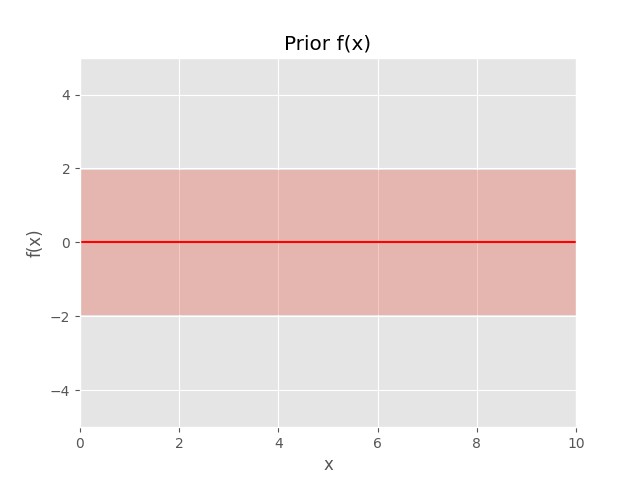
\includegraphics[width=\textwidth]{figures/introduction-gp/prior.png}
        \caption{Prior}
        \label{fig:gp_prior}
    \end{subfigure}
    \begin{subfigure}{0.49\textwidth}
        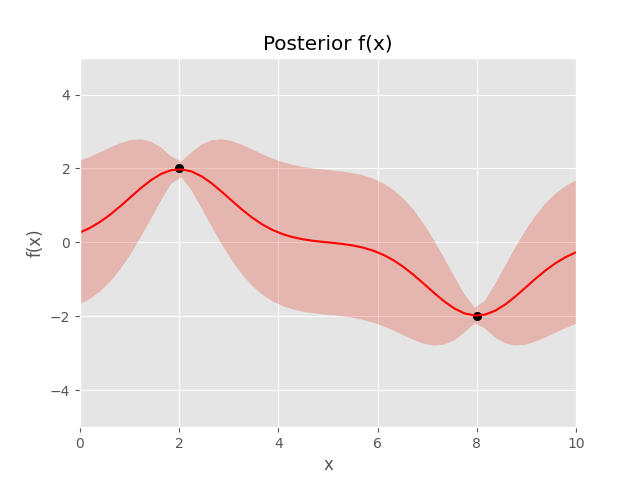
\includegraphics[width=\textwidth]{figures/introduction-gp/posterior.png}
        \caption{Posterior after observing the function at two different inputs (black dots).}
        \label{fig:gp_posterior}
    \end{subfigure}
    \caption{Simple Gaussian Process example with zero-mean and \acrshort{rbf} kernel with unit variance. The red line is the mean, while the red area is the $95\%$ confidence interval.}
    \label{fig:gp_simple}
\end{figure}

\section{Vector-valued Gaussian Process}\label{sec:theory_vector_gp}
\acrshort{gp}s can easily be extended for vector-valued functions by simply considering the joint distribution of each function component as in \cref{eq:gp_vector}.
\begin{equation}\label{eq:gp_vector}
     \vec{f}(\boldsymbol{x}) = \begin{bmatrix} f_x (\boldsymbol{x})\\ f_y (\boldsymbol{x})\end{bmatrix} \sim \text{GP} \big(\begin{bmatrix} m_x(\boldsymbol{x})\\m_y(\boldsymbol{x})\end{bmatrix}, \ \begin{bmatrix}
    k_{xx}(\boldsymbol{x}, \boldsymbol{x}') & k_{xy}(\boldsymbol{x}, \boldsymbol{x}') \\ k_{xy}(\boldsymbol{x}, \boldsymbol{x}')^\intercal & k_{yy}(\boldsymbol{x}, \boldsymbol{x}')
    \end{bmatrix}\big) 
\end{equation}

Only independent output dimensions, i.e. $k_xy = k_yx = 0$ will be considered in this thesis to reduce the number of complicating factors. This is, however, not without consequences as it assumes zero covariance between the two outputs. This issue is revisited in \cref{chap:discussion}.

\section{Kernels}\label{sec:kernels}
This section will introduce some relevant kernels for this thesis. Many more kernels are available in the literature \cite{rasmussen}.  
\subsection{Stationary Kernels}
Stationary kernels are kernels which only depends on $\boldsymbol{r} = \boldsymbol{x} - \boldsymbol{x'}$ and is usually specified as a function of a single variable.
\subsubsection{Constant Kernel}
As the name implies, the constant kernel is a kernel that is independent of the input. It is typically used as a scaling parameter in combination with other kernels.

\begin{equation}
    k(\boldsymbol{\cdot}) = \sigma^2
\end{equation}

\subsubsection{White kernel}
The \textit{White Kernel} is useful for modeling whitenoise in a system as \acrshort{iid} \cite{scikit-learn}. The white kernel is given by
\begin{equation}
    k(\boldsymbol{x}_i, \boldsymbol{x}_j) = \delta_{ij} \sigma^2
\end{equation}
where $\delta_{ij}$ is the Kronecker-delta which is $1$ if $i=j$ and $0$ otherwise. This is the same as the noise term added in \cref{alg:gp_prediction}.

\subsubsection{Radial Basis Function}\label{sec:kernels_rbf}
The \textit{\acrfull{rbf}} kernel, also referred to as \textit{squared exponential kernel}, is one of the most frequently used kernels, and is given by the covariance function in \cref{sec:kernels_rbf}. The scaling parameter $l$ is the \textit{charactheristic length scale} and can intuitively be thought of as a smoothness parameter. This kernel yields infinitely differentiable functions, meaning that any function drawn from a \acrshort{gp} with this kernel is very smooth\cite{rasmussen}.
\begin{equation}\label{eq:kernel_rbf}
    k(\boldsymbol{r}) = \exp \big\{-\frac{||\boldsymbol{r}||^2}{2 l^2}\big\}
\end{equation} 

\subsubsection{Matérn class}
The \textit{Matérn Class} of kernels is given by the covariance function in \cref{eq:kernel_matern}, where $K_v$ is the \textit{modified Bessel function}. 

\begin{equation}\label{eq:kernel_matern}
    k(\boldsymbol{r}) = \frac{2^{1-\nu}}{\Gamma(\nu)}\bigg(\frac{\sqrt{2 \nu} ||\boldsymbol{r}||}{l} \bigg)^\nu K_\nu \bigg(\frac{\sqrt{2\nu} || \boldsymbol{r}||}{l} \bigg)
\end{equation}
The parameter $\nu > 0$ determines the smoothness, where:
\begin{itemize}
    \item $\nu=\frac{1}{2}$ yields the \textit{Ornstein-Uhlenbeck Process} and functions, that when drawn from a \acrshort{gp}, are continious, but not differentiable. The kernel is equivalent to $$k(\boldsymbol{r}) = \exp \big\{-\frac{||\boldsymbol{r}||}{l}\big\}$$
    \item $\nu=\frac{3}{2}$ yields functions that, when drawn from a \acrshort{gp}, are continous and once-differentiable. The kernel is equivalent to $$k(\boldsymbol{r}) = \big(1 + \frac{\sqrt{3} ||\boldsymbol{r}||}{l}\big) \exp\big\{- \frac{\sqrt{3} ||\boldsymbol{r}||}{l}\big\}$$
    \item $\nu=\frac{5}{2}$ yields functions, that when drawn from a \acrshort{gp},  are continous and twice differentiable. The kernel is equivalent to $$k(\boldsymbol{r}) = \big(1 + \frac{\sqrt{5} ||\boldsymbol{r}||}{l} + \frac{5 ||\boldsymbol{r}||^2}{3 l^2}\big) \exp\big\{- \frac{\sqrt{5} ||\boldsymbol{r}||}{l}\big\}$$
\end{itemize}
More generally, the functions drawn from a \acrshort{gp} with a Matérn class kernel, is $k$-times differentiable if and only if $\nu > k$\cite{rasmussen}. The Matérn class of kernels is argued to be a better choice than the \acrshort{rbf} kernel for many physical systems, as the infinitely smooth function generated by \acrshort{rbf} is too smooth \cite{rasmussen}.
Further mathematical details can be found in \cite[sec.~4.2]{rasmussen} as it is outside the scope of this thesis.


\subsection{Combining multiple kernels}
Kernels can be mixed and matched through multiplication and addition, where the behavior of the individual kernels can be combined to describe more complex functions. A simple example is using the constant kernel to scale the covariance of other kernels. Different kernels can also be used for each input dimension.
\section{Hyperparameter selection}
Manually tuning the kernel hyperparameters is tedious and time-consuming, motivating the need for automatic selection of parameters. This section will discuss an automated approach for hyperparameter selection with \acrshort{gp}s.

\subsection{Maximum Likelihood - The Marginal Likelihood}\label{sec:gp_mle}
The \textit{marginal likelihood}, which is the likelihood of observing a set of given observations $\boldsymbol{y}$, conditioned on a \acrshort{gp} with kernel parameters $\boldsymbol{\theta}$ and inputs $X$, is given by 

\begin{equation}
    p(\boldsymbol{y} \; | \; X, \boldsymbol{\theta}) = \mathcal{N}\big(\boldsymbol{y} \; | \; \boldsymbol{m}(X), K_{\boldsymbol{\theta}}(X, X)\big)
\end{equation}
and can be used to obtain a \textit{\acrfull{ml}} estimate of the parameters $\boldsymbol{\theta}$.
Defining $\tilde{\boldsymbol{y}} \triangleq \boldsymbol{y} - \boldsymbol{m}(X)$ and taking the logarithm yields \cref{eq:gp_log_marginal_likelihood} 
\begin{tcolorbox}[ams align, title={Log Marginal Likelihood}]\label{eq:gp_log_marginal_likelihood}
    \begin{split}
    \log p(\boldsymbol{y} \; | \; X, \boldsymbol{\theta}) = &-\frac{1}{2} \tilde{\boldsymbol{y}}^\intercal K_{\boldsymbol{\theta}}(X, X)^{-1}\tilde{\boldsymbol{y}} - \frac{1}{2} \log |K_{\boldsymbol{\theta}}(X, X)| \ldots\\ &- \frac{n}{2} \log (2 \pi)
    \end{split}
\end{tcolorbox} where the optimal hyperparameters $\boldsymbol{\theta}_{\text{ML}}$ can be found by maximizing this quantity\footnote{
    The marginal likelihood is generally not a convex function of $\boldsymbol{\theta}$ as the kernel functions are usually non-linear functions of $\boldsymbol{\theta}$, and multiple local optima may exist. The practical effects include that the observed data may be explained well by different combinations of parameters, and each combination serves as a distinct interpretation of the data. During optimization, care should be taken to avoid a bad local optimum \cite{rasmussen}.}, i.e.
\begin{equation}
    \boldsymbol{\theta}_{\text{ML}} = \arg \max_{\boldsymbol{\theta}} \log p(\boldsymbol{y} \; | \; X, \boldsymbol{\theta}) = \arg \min_{\boldsymbol{\theta}} \big(- \log p(\boldsymbol{y} \; | \; X, \boldsymbol{\theta})\big)
\end{equation}

The name marginal likelihood comes from the fact that the latent function $\boldsymbol{f}$ is marginalized out, i.e. the parameters are optimized over all possible latent functions $\boldsymbol{f}$.

\begin{equation}
    p(\boldsymbol{y} \; | \; X, \boldsymbol{\theta}) = \int_{\boldsymbol{f}} p\big(\boldsymbol{y} \;| \; \boldsymbol{f}\big) p\big(\boldsymbol{f} \; |\; m(X), K(X, X)\big) d\boldsymbol{f}
\end{equation}

The marginal likelihood is somewhat resilient to overfitting, as it naturally incorporates a trade-off between model complexity and model fit. However, the optimization step always imposes the risk of overfitting, especially if there are many hyperparameters \cite{rasmussen}. 

Optimizing \cref{eq:gp_log_marginal_likelihood} with gradient descent requires the inversion of the kernel matrix at each iteration. It quickly becomes a costly operation, limiting the size of the dataset that can be used realistically. A possible solution to this problem is to approximate the global \acrshort{gp} by several local models, as proposed in work such as \cite{paralell_gp_mle,paralell_gp_mle_2}. These smaller \acrshort{gp} models can then be evaluated in parallel and collaborate in the search for a global optimum. 

\section{Sampling from a Gaussian Process}\label{sec:gp_samples}
As the \acrshort{gp} is a joint Gaussian distribution, random samples can be drawn from it as with any other multivariate Gaussian.

\begin{equation}\label{eq:gp_samples}
    \boldsymbol{f}_* \sim \mathcal{N}(\bar{\boldsymbol{f}}_*, \mathbb{V}[\boldsymbol{f}_*])
\end{equation}

More specifically, a vector of \acrshort{iid} standard normal samples, $Z$, can be turned into samples from a joint Gaussian distribution.

Once again, the Cholesky decomposition is used to decompose the \acrshort{gp} covariance, i.e. $\mathbb{V}[\boldsymbol{f}_*] = L L^\intercal$. Using $L$ and $\bar{\boldsymbol{f}}_*$, \cref{eq:gp_samples} can be expressed as 
\begin{equation}
    \mathcal{N}(\bar{\boldsymbol{f}}_*, \mathbb{V}[\boldsymbol{f}_*]) = \bar{\boldsymbol{f}}_* + L \mathcal{N}(0, I)
\end{equation}
which yields a way to convert indendent standard normal samples into samples from a \acrshort{gp} \cite{rasmussen}:

\begin{equation}
    \boldsymbol{f}_* = \bar{\boldsymbol{f}}_* + L Z, \quad Z \sim \mathcal{N}(0, I)
\end{equation}

\section{Standardization}
The method of \textit{standardization}\todo[]{find source} is the process of converting the data into a standard unit of measurement, which in practice involves transforming the data to have zero mean and unit variance. This is useful when comparing measures of different scales.

The proposed \acrshort{gp} implementation works well with and without standardized input data, but standardization has one crucial benefit. While the current implementation allows separate kernel hyperparameters for each input dimension in $\boldsymbol{x}$, the kernel is assumed to be identical for each output of $\vec{f}$. The kernel therefore represents the variability of \textbf{both} output dimensions at once. However, with standardized training outputs $Y$, the kernel is relative to the standard deviation of the training data. This way, the \acrshort{gp} can express the different levels of uncertainty for each output dimension while still sharing the same kernel. An even more flexible approach would be to allow separate kernels for each dimension, though at the cost of more complex hyperparameter tuning.

\section{Approximate methods}
The standard derivation of the \acrshort{gp} requires inverting the kernel matrix, either through the Cholesky Decomposition or directly. Unfortunately, the computational complexity is $\frac{n^3}{6}$ operations for the Cholesky Decomposition and similarly $\frac{n^2}{2}$ for solving triangular systems \cite{rasmussen}. This may be acceptable for sparse datasets, but it makes \acrshort{gp}s infeasible for Big Data applications. 

For simple functions, it often works well to only use a representable subset of the data. However, throwing away the majority of available data is not an elegant solution to the problem. 

\subsection{Reduced-rank approximation}

Several approximations are discussed in \cite{rasmussen} and typically use a \textit{reduced-rank approximation} of the kernel matrix $K=Q Q^\intercal$ with $Q \in \mathcal{R}^{n \times q}$, and use the \textit{matrix inversion lemma} \cite[p.~201]{rasmussen}, reducing the inversion of the $n \times n$ matrix to the inversion of a $q \times q$ matrix instead. Unfortunately, the optimal reduced-rank approximations depend on the eigenvalue decomposition, which itself is a $\mathcal{O}(n^3)$ operation. However, if a cheap approximation to the eigenvalue decomposition can be found, it can potentially be used to approximate the \acrshort{gp}. One such low-rank approximation is the Nyström method, where a subset of the dataset is used to approximate the eigenvalues.    

\subsection{Sparse Variational Gaussian Process}

To deal with the computational complexity of \acrshort{gp}s, \cite{Titsias2008VariationalMS} introduced the \textit{\acrfull{svgp}}. Rather than directly using all the available training data directly, one can instead attempt to summarize the data $(X, \boldsymbol{y})$ using a set of $m$ \textit{inducing variables} for the latent function values $\boldsymbol{f}_m$ at the inducing points $X_m$. $X_m$ can either be a subset of the available training inputs $X$ or auxiliary \textit{pseudo-points}. The goal of \acrshort{svgp} is then to infer the inducing points $X_m$ as well as the hyperparameters $\boldsymbol{\theta}$ from data. 


\section{The Kalman Filter}


\chapter{Historical AIS data}\label{chap:ais}

The \textit{\acrfull{ais}} is a vessel-to-vessel communication system, which allows a vessel to share vital information about its current state with other ships, base stations, and satellites electronically. International voyaging ships with gross tonnage larger than 300 and all passenger ships are required to install an \acrshort{ais} transceiver according to the \textit{Safety Of Life At Sea} (SOLAS) convention \cite{ais_wiki}

The typical \acrshort{ais} receiver has a range of about 10-20 nautical miles. However, \acrshort{ais} transceivers have been installed on satellites in later years, resulting in global coverage. The messages are divided into two types of classes:
\begin{description}
    \item[Class A] typically transmits at a higher rate, ranging between 30 times per minute for high-velocity vessels to every third minute for vessels at rest. 
    \item[Class B] are typically smaller, cheaper, and simpler than their Class A counterparts. The position message for Class B is sent every 3 minutes when the vessel's speed is less than 2 knots and every 30 seconds for faster speeds. 
\end{description}

\section{Message Contents}
\begin{table}[h]
    \centering
    \begin{tabular}{p{0.15\textwidth}  p{0.8\textwidth}}
        \textit{\textbf{Parameter}} & \textit{\textbf{Explanation}}                                                                                                     \\ \hline
        IMO                         & 7 digit vessel identification number that remains unchanged when transferring a vessel's registration to a new country            \\
        \acrshort{mmsi}                        & \textit{\acrfull{mmsi}}, a 9 digit vessel identification number                                                          \\
        Long                        & Degrees longitude in range $[-180^\circ W, 180^\circ E]$                                                                          \\
        Lat                         & Degrees latitude in range $[90^\circ S, 90^\circ N]$                                                                             \\
        \acrshort{cog}                         & \textit{\acrfull{cog}} is the clockwise rotation of the vessel's velocity vector relative to true north                               \\
        \acrshort{sog}                         & \textit{\acrfull{sog}} is the absolute value of the vessel's velocity vector in knots.                                               \\
        Heading                     & Direction of vessel's nose or bow relative to true north. Independent of the actual movement, so not necessarily identical to COG. NB: Not always available. \\
        Timestamp                   & Number of days elapsed since 1. jan 1900, 00:00                                                                                   \\ \hline
    \end{tabular}
    \caption{Common content of \acrshort{ais} messages \cite{hexeberg}.}
    \label{table:ais_content}
\end{table}
The typical \acrshort{ais} message contains unique identification (MMSI / IMO), position (longitude and latitude GPS coordinates), course (\acrshort{cog}) and speed (\acrshort{sog}). The relevant message content for this thesis is summarized in \cref{table:ais_content}.

Several other fields may additionally be available, depending on the transceiver and which information the crew has entered. 

\section{The Dataset}
The total dataset contains $2995644$ \acrshort{ais} samples collected between 1. Jan and 31. Des 2015. There are $1555$ unique \acrshort{mmsi} values, though most of the messages come from a small subset of the vessels. More than $80\%$ of the dataset originates from the top $250$ vessels, as seen in \cref{fig:ais_cdf}.

\begin{figure}[h]
    \centering
    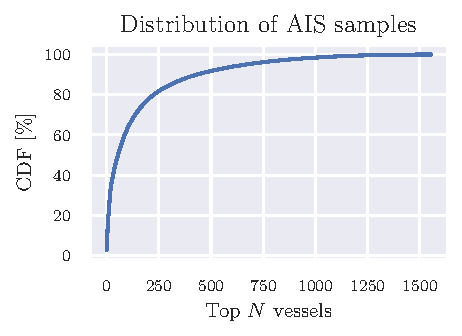
\includegraphics[width=0.5\textwidth]{figures/mmsi_cdf.pdf}
    \caption{Cumulative distribution of \acrshort{ais} messages for the $N$ most frequent vessel's.}
    \label{fig:ais_cdf}
\end{figure}

However, the dataset is currently too large to conveniently work with on a single computer. Two local regions are instead used in this thesis, and they are shown in \cref{fig:ais_data}. The first subset is from a curved section of the Trondheim fjord with a lot of traffic. The subset also includes a ferry crossing, which crosses the traffic lane. The other subset is from deeper into the fjord, from a relatively straight section. The dataset therefore contains both straight-line and curved trajectories, as well as crossing trajectories. 

\begin{figure}
    \centering
    \begin{subfigure}{\textwidth}
        \centering
        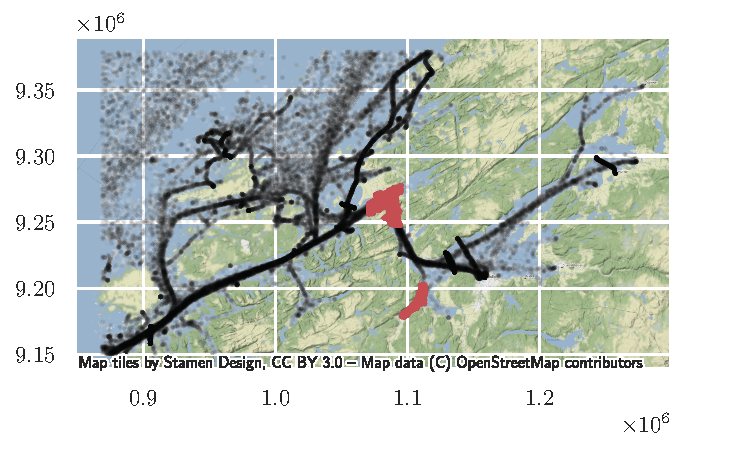
\includegraphics{figures/ais_map.pdf}
        \caption{Full dataset. The blue areas mark the subset that will be used for testing purposes.}
    \end{subfigure}
    \begin{subfigure}{\textwidth}
        \centering
        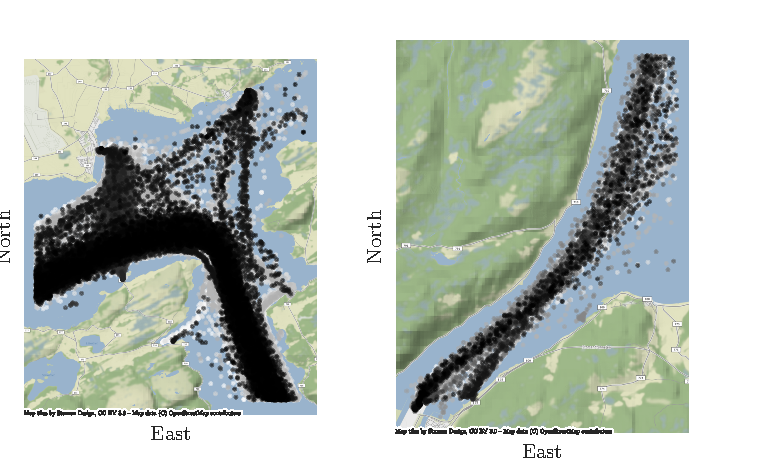
\includegraphics{figures/ais_map_zoom.pdf}
        \caption{Zoomed-in version of the subsets used in this thesis. The blue subset in the left-most map shows the \acrshort{ais} data from three local ferries, which make out more than half of the dataset.}
    \end{subfigure}
    \caption{The available \acrshort{ais} data used in this thesis. }
    \label{fig:ais_data}
\end{figure}

\section{Scenario}
The \acrshort{ais} dataset contains samples from a wide variety of different trajectories, as each trajectory is the result of a vessel's intention, be it reaching a specific destination, commercial fishing, or simply for leisure. As a result, there is a wide range of possible overlapping trajectories that a vessel might follow in any given area. Therefore, this thesis will narrow the problem of long-term prediction down to prediction in specific \textit{scenarios}. A scenario is in this thesis characterized by the vessel's initial position, speed and course, and it is assumed that vessels in a given scenario tend to follow similar trajectories. Though not used in this thesis, it would also be natural to incorporate contextual information such as vessel type, as there is likely quite a lot of variability between the behavior of different types of vessels. 

When predicting the trajectory for a given target vessel, only the subset of \acrshort{ais} messages from similar situations will be used. This simplifying assumption is a critical part of all methods proposed in this thesis. It allows the \acrshort{ais} to be reduced significantly for any given prediction and is what makes the methods computationally feasible. The following requirements must be satisfied for a trajectory to qualify as being in a similar scenario as the target vessel:
\begin{enumerate}
    \item The trajectories' initial position must be close to the target vessel's position $\boldsymbol{x}$. A fixed threshold at $\boldsymbol{x} \pm \Delta \boldsymbol{x}$ is used.
    \item The trajectories' initial \acrshort{cog} must be close to the target vessel's heading $\mathcal{X}$. A fixed threshold at $\mathcal{X} \pm \Delta \mathcal{X}$ is used.
    \item The trajectories' initial \acrshort{sog} must be close to the queried velocity $v$. A fixed threshold at $v \pm \Delta v$ is used.
\end{enumerate}


The notion of only using a small subset of close-by samples from the \acrshort{ais} data is somewhat similar to the SPNS method proposed by \cite{Hexeberg2017AISbasedVT}, though a key distinction is that this thesis selects entire trajectories based on the initial conditions, rather than individual points. 

\subsection{Clustering}
In practical applications, it may be beneficial to use a fixed number of scenarios. For example, clustering-based methods may be used to cluster similar trajectories into a fixed number of scenarios. This approach is not implemented in this thesis but is considered a natural next step.


\section{Preprocessing}
The position (longitude and latitude) is converted from the standard World Geodetic System (WGS84) coordinates into the EUREF89 UTM32 (EPSG-25832) coordinate system \cite{kartverket}.  As a result, the coordinates are converted from spherical coordinates to a 2D euclidian coordinate system, where the first and second axis corresponds to easting and northing, respectively. This coordinate system is one of two official coordinate systems in Norway and yields significantly better projections in this area than other alternatives, such as the Web-Mercator projector frequently used by online maps. Zone 32 is selected as it encompasses the target region.

\subsection{From samples to trajectories}\label{sec:from_ais_to_traj}
Samples with identical \acrshort{mmsi} and less than $15$ minutes between subsequent samples are considered part of the same trajectory. The $15$ minute requirement is added to ensure that samples before and after docking are considered separate trajectories. The length of the trajectories must be between $15$ and $30$ minutes, and the number of samples in each trajectory must be greater than $4$. 

\chapter{Model trajectories directly using a Gaussian Process}\label{chap:direct_gp}
 A tempting solution is to directly apply the \acrshort{gp} framework introduced in the previous chapter and model the vessel's trajectory as a function of time $\vec{f}(\tau)$. However, as there are no observations of the target vessel's future position, there is no actual data to condition the \acrshort{gp} on. Instead, this chapter will attempt to use nearby trajectories and assume these historical trajectories resemble the future trajectory of the target vessel. 

\section{Method}
While a pure function of time is tempting, it is unable to differentiate between different historical trajectories. To utilize as much of the available information in a single \acrshort{ais} message as possible, a bit more complex formulation $\vec{f}(\boldsymbol{x}_0, \psi_0, v_0, \tau): \mathcal{R}^5 \to \mathcal{R}^2$ is proposed instead to compensate for any initial differences in position, velocity or course of nearby trajectories. The key variables are explained in \cref{table:posgp_key_variables}.

\begin{table}[h]
    \centering
    \begin{tabular}{ll}
        \textit{\textbf{Variable}}              & \textit{\textbf{Description}}      \\ \hline
        $\boldsymbol{x}_0 \in \mathcal{R}^2$    & Trajectorys initial position       \\
        $\mathcal{X}_0 \in [0, 360)$            & Trajectorys initial \acrshort{cog} \\
        $v_0 \in \mathcal{R}$                   & Trajectorys initial \acrshort{sog} \\
        $\tau \in [0, \infty)$                  & Prediction timestamp               \\
        $\boldsymbol{x}_\tau \in \mathcal{R}^2$ & Predicted position                 \\
    \end{tabular}
    \caption{Key variables}
    \label{table:posgp_key_variables}
\end{table}
The method is formulated in mathematical terms in \cref{eq:gp_direct}. This will from now on be referred to as the \textit{Direct \acrshort{gp}} approach, as it directly utilizes a \acrshort{gp} to predict the trajectory.

\begin{subequations}\label{eq:gp_direct}
    \begin{align}
        \boldsymbol{f}(\boldsymbol{\eta}) & = \boldsymbol{x}_{\tau} \label{eq:gp_direct_f}, \quad \boldsymbol{\eta} = \begin{bmatrix} \boldsymbol{x}_0 & \psi_0 & v_0 & \tau\end{bmatrix}                   \\
        \boldsymbol{f}(\boldsymbol{\eta}) & \sim \text{GP}(\boldsymbol{m}(\boldsymbol{\eta}), K(\boldsymbol{\eta}, \boldsymbol{\eta}))\label{eq:gp_direct_f_dist}
    \end{align}
\end{subequations}

The function $\vec{f}$ can be conditioned on similar trajectories using \cref{alg:gp_prediction} from \cref{chap:theory}, and then be used to answer queries about the likely trajectories the vessel might follow.

\subsection{Key Assumption}
This formulation builds on the key assumption that the target vessel is following the same underlying trajectory as the nearby historical trajectories. In other words, the function $\vec{f}$ does not represent the target vessel's future trajectory; it merely interpolates the past trajectories with similar initial conditions. 


%The conceptual benefits of this formulation include:
%\begin{description}
%    \item[Continuous formulation] The model directly models the position at any time $\tau$ and does not require discretization. It can therefore be queried for any continuous timestamp $\tau$.
%    \item[Conceptually easy] This formulation directly expresses the unknown trajectory, making it conceptually simple to understand.
%    \item[Simple Problem formulation] The model requires few components and builds directly on the \acrshort{gp}s introduced in \cref{chap:theory}.
%    \item[Easy incorporation of available AIS data] The reported \acrshort{cog} and \acrshort{sog} can easily be incorporated into the similarity measure, utilizing more of the available data.
%\end{description}

\subsection{Choice of Kernel}
Many different kernels may work well with this formulation. This section will cover a few alternatives that worked well in practice, but there are likely many other alternatives that may work just as well, if not better. 

The \acrshort{rbf} kernel was found to work well with the formulation used in this chapter. Along the traffic lanes, vessels tend to move in a smooth trajectory, which makes the \acrshort{rbf} kernel a good choice. As the function arguments are of different scales, it is a good idea to use different lengthscales for each input dimension, i.e.

\begin{equation}
    k(\boldsymbol{\eta}, \boldsymbol{\eta}') = \sigma^2 \exp \big[ (\boldsymbol{\eta} - \boldsymbol{\eta}') W^{-1} (\boldsymbol{\eta} - \boldsymbol{\eta})^\intercal \big]
\end{equation}
where $W$ is a diagonal matrix with a separate lengthscale for each dimension and $\sigma^2$ is a scale parameter. This kernel yields smooth functions for $\vec{f}$ and is well suited to model the general trend of the trajectory.

In some scenarios, a single \acrshort{rbf} kernel result in an unreasonably smooth function. Adding a second \acrshort{rbf} kernel as in \cref{eq:direct_gp_kernel} work well in these scenarios as it gives the model some additional flexibility in local regions. However, it makes hyperparameter selection significantly more complicated as the optimal solution is no longer unique.  

\begin{equation}\label{eq:direct_gp_kernel}
    k(\boldsymbol{\eta}_i, \boldsymbol{\eta}_j) = \sigma_0 k_0(\boldsymbol{\eta}_i, \boldsymbol{\eta}_j) + \sigma_1 k_1(\boldsymbol{\eta}_i, \boldsymbol{\eta}_j)
\end{equation}

Each term in this kernel offer a unique interpretation:
\begin{description}
    \item[Long term trend $k_0$] is a \acrshort{rbf} kernel intended to cover the long-term behavior of the trajectories, i.e., a smooth component describing the overall trend of the trajectories. The length scales of this kernel are expected to be relatively large.
    \item[Dependent noise $k_1$] is a \acrshort{rbf} kernel intended to model the local variations between different trajectories which is not well explained by $k_0$. The length scales are therefore expected to be short.
\end{description}

\section{Implementation Details}

The main concern with this formulation is the significant computational complexity of conditioning $\vec{f}$ on a large number of samples. As it is infeasible to fit the entire \acrshort{ais} dataset to a single \acrshort{gp}, multiple smaller \acrshort{gp}s will be used instead. This raises the question, how should the training data be assigned to each \acrshort{gp}?

\subsection{Selecting representable trajectories for training}
The key observation is that only a small subset of the \acrshort{ais} samples is relevant for any given input query. Trajectories with significantly different initial conditions will get a negligible covariance. Hence, only a small subset of the trajectories has any effect on the prediction. 

\subsection{Clustering}
In practical applications, it may be beneficial to avoid recomputing the \acrshort{gp} for each new query. Instead, clustering-based methods may be used to create a cluster of similar trajectories and instead fit \acrshort{gp}s for each cluster. This approach is not implemented in this thesis but is considered a natural next step.


\subsection{Approximate Gaussian Process}
Another promising approach is to utilize an approximation technique to avoid the scalability issue of \acrshort{gp}s. Though not implemented in this thesis, the \acrshort{svgp} introduced in \cref{chap:theory} is one such method that attempts to fit a \acrshort{gp} while simultaneously finding a good subset of the data to summarize the full dataset.


\chapter{GP-EKF: Non-parametric dynamic system using AIS tracking data}\label{chap:gp_ekf}
One of the significant issues with the direct approach is the unimodal assumption of using a \acrshort{gp}. It works well as long as vessels agree on a specific trajectory, but fails as soon as there are multiple branching trajectories. To solve this problem, a non-parametric dynamical model is proposed in this chapter and is used to simulate vessel trajectories. This chapter is inspired by \cite{pedestrian,gpekf,vehicle_gp_prediction,multistep_gp}.



The vessel trajectory $\boldsymbol{\mathcal{T}}$ can be expressed using the dynamical system
\begin{subequations}
    \begin{align}
        \boldsymbol{x}_{t+1}       & = \boldsymbol{x}_t + \vec{f}(\boldsymbol{x}_t,\tau_t)                       \\
        \boldsymbol{\mathcal{T}}_t & = \boldsymbol{x}_t + \epsilon, \quad \epsilon \sim \mathcal{N}(0, \sigma^2)
    \end{align}
\end{subequations}
The function $\vec{f}(\cdot): \mathcal{R}^3 \to \mathcal{R}^2$ denotes the vector field describing the expected velocity. In the case of long-term prediction, the dynamics $\vec{f}(\cdot)$ are unknown and unlikely to be stationary. Instead of using the usual parametric approaches to ODE models, the goal of this chapter is to use a \acrshort{gp} to create a non-parametric representation of the dynamics $\vec{f}(\cdot)$ by learning from historical trajectories of other vessels. This way, arbitrary complex dynamics can be learned without being limited by a fixed parametrization. The \acrshort{gp} considered in this chapter is a vector-valued \acrshort{gp} with zero mean and identical kernel for each output dimension, as expressed in \cref{eq:gp_vec_field}. The output dimensions are assumed to be independent.

\begin{equation}\label{eq:gp_vec_field}
    \vec{f}(\boldsymbol{x}, t) = \vec{f}(\boldsymbol{\eta}) = \begin{bmatrix} f_E (\boldsymbol{\eta})\\ f_N (\boldsymbol{\eta})\end{bmatrix} \sim \text{GP} \big(0 , \; k(\boldsymbol{\eta}, \boldsymbol{\eta}')\big)
\end{equation}

The pipeline for making predictions using available \acrshort{ais} data will now be introduced in greater detail, but can be summarized as:
\begin{enumerate}
    \item Calculate trajectory gradients $\boldsymbol{y}$ for inputs $\boldsymbol{\eta}$ from available \acrshort{ais} data.
    \item Fit a \acrshort{gp} to the time-varying vector-field $\vec{f}: \mathcal{R}^3 \to \mathcal{R}^2$
    \item Simulate the vessel as it is moving through the vector field $\vec{f}$, using either \acrshort{ekf}-based prediction or Sequential Monte Carlo.
\end{enumerate}



\section{Notation and variables}
The key variables for this chapter are summarized in \cref{table:dyngp_key_variables}. All other variables will be introduced as needed.
\begin{table}[h]
    \centering
    \begin{tabular}{ll}
        \textit{\textbf{Variable}}               & \textit{\textbf{Description}}                                      \\ \hline
        $\boldsymbol{x}_t \in \mathcal{R}^2$     & Vessel position at step $t$                                        \\
        $\tau_t \in \mathcal{R}$                 & Timestamp at step $t$, number of seconds since start of trajectory \\
        $\mathcal{X}_t \in [0, 360)$             & Vessel's course over ground in degrees at step $t$                 \\
        $v_t \in \mathcal{R}$                    & Vessel's speed over ground in knots at step $t$                    \\
        $\boldsymbol{P}_t \in \mathcal{R}^{2x2}$ & State Covariance at step $t$                                       \\
    \end{tabular}
    \caption{Key variables}
    \label{table:dyngp_key_variables}
\end{table}

Note that throughout this chapter, some of the notation used in \cref{sec:gp} will be relaxed in order to reduce the notational complexity. More specifically, the \acrshort{gp}s in this chapter are always assumed to be conditioned on available data, i.e. $p\big(\vec{f}(\boldsymbol{x})\big) = p\big(\vec{f}(\boldsymbol{x}) \; | \; \boldsymbol{y} \big)$.

\section{Simulating Trajectories}

The vector-field $\vec{f}$ can be expressed using the \acrshort{gp} framework from \cref{chap:theory} to get the prediction model
\begin{equation}\label{eq:dyngp_predictive_distribution}
    p(\boldsymbol{x}_{t+1} | \boldsymbol{x}_t) = \mathcal{N}\big(\boldsymbol{x}_{t+1} \; | \; (\boldsymbol{x}_t + \mathbb{E}[\vec{f}(\boldsymbol{x_t})]), \mathbb{V}[\vec{f}(\boldsymbol{x}_t, \tau_t)] \big)
\end{equation}

Given a current estimate $p(\boldsymbol{x}_t)$, the marginal next state distribution for the predicted state then becomes
\begin{equation}\label{eq:dyngp_true_posterior}
    p(\boldsymbol{x}_{t+1}) = \int_{\boldsymbol{x}_t} p(\boldsymbol{x}_{t+1} | \boldsymbol{x}_t) p(\boldsymbol{x}_t) d\boldsymbol{x}_t
\end{equation}

However, this integral is intractable, as both the mean and variance depend on the current state $\boldsymbol{x}_t$ with non-trivial relationships \cite{pedestrian,multistep_gp}. A solution to this problem is to use sampling-based methods, and one such approach is discussed later in \cref{sec:dyngp_particle}.
However, the main method proposed in this chapter will approximate this integral by making a few simplifying assumptions. The integral can be approximated by assuming that the posterior distribution is Gaussian, and the mean and variance can be calculated using the law of iterated expectations and conditional variance \cite{multistep_gp}. Assuming the current estimate to be distributed according to the Gaussian distribution $p(\boldsymbol{x}_t) = \mathcal{N}(\bar{\boldsymbol{x}}_t, \boldsymbol{P}_t)$, the mean and variance of $\boldsymbol{x}_{t+1}$ is given by

\begin{subequations}\label{eq:gp_prediction_mean_variance}
    \begin{align}
        \begin{split}
            \mathbb{E}[\boldsymbol{x}_{t+1}] &= \mathbb{E}\big[ \mathbb{E}[\boldsymbol{x}_{t+1} | \boldsymbol{x}_t] \big]\\
            &= \mathbb{E}\big[ \boldsymbol{x}_t + \mathbb{E}[\vec{f}(\boldsymbol{x}_t, \tau_t) | \boldsymbol{x}_t] \big]\\
            & = \bar{\boldsymbol{x}}_t + \mathbb{E}\big[ \mathbb{E}[\vec{f}(\boldsymbol{x}_t, \tau_t) | \boldsymbol{x}_t] \big]
        \end{split} \\
        \begin{split}
            \mathbb{V}[\boldsymbol{x}_{t+1}] &= \mathbb{E}\big[\mathbb{V}[\boldsymbol{x}_{t+1} | \boldsymbol{x}_t]\big] + \mathbb{V}\big[ \mathbb{E}[\boldsymbol{x}_{t+1} | \boldsymbol{x}_t] \big]\\
            &= \mathbb{E}\big[\mathbb{V}[\vec{f}(\boldsymbol{x}_t, \tau_t) | \boldsymbol{x}_t]\big] + \mathbb{V}\big[\boldsymbol{x}_t + \mathbb{E}[\vec{f}(\boldsymbol{x}_t, \tau_t) | \boldsymbol{x}_t] \big]
        \end{split}
    \end{align}
\end{subequations}

The mean and variance of the \acrshort{gp} are the same conditional mean and variance as in \cref{eq:gp_conditional_simple} from \cref{chap:theory}, which both are non-linear functions of $\boldsymbol{x}_t$. A first-order Taylor approximation around the current best estimate $\bar{\boldsymbol{x}}_t$ is then applied to linearize the \acrshort{gp} mean and variance, with respect to $\boldsymbol{x}_t$.

\begin{subequations}\label{eq:gp_predict_taylor_approx}
    \begin{align}
        \mathbb{E}[\vec{f}(\boldsymbol{x}_t) | \boldsymbol{x}_t)]    & \approx \mathbb{E}[\vec{f}(\bar{\boldsymbol{x}}_t, \tau_t)] +  \frac{\partial  \mathbb{E}[\vec{f}(\boldsymbol{x}_*, \tau_t)]}{\partial \boldsymbol{x}_*}\bigg|_{\boldsymbol{x}_* = \bar{\boldsymbol{x}}_t} (\boldsymbol{x}_t - \bar{\boldsymbol{x}}_t) \\
        \mathbb{V}[f(\boldsymbol{x}_{t}, \tau_t) | \boldsymbol{x}_t] & \approx \mathbb{V}[\vec{f}(\bar{\boldsymbol{x}}_t, \tau_t)] +  \frac{\partial \mathbb{V}[\vec{f}(\boldsymbol{x}_*, \tau_t)]}{\partial \boldsymbol{x}_*}\bigg|_{\boldsymbol{x}_* = \bar{\boldsymbol{x}}_t} (\boldsymbol{x}_t - \bar{\boldsymbol{x}}_t)
    \end{align}
\end{subequations}


Defining temporary variables for the Jacobians
\begin{align}
    \boldsymbol{U}_t & \triangleq \frac{\partial  \mathbb{E}[\vec{f}(\boldsymbol{x}_*, \tau_t)]}{\partial \boldsymbol{x}_*}\big|_{\boldsymbol{x}_* = \bar{\boldsymbol{x}}_t} & \boldsymbol{V}_t & =\frac{\partial \mathbb{V}[\vec{f}(\boldsymbol{x}_*, \tau_t)]}{\partial \boldsymbol{x}_*}\big|_{\boldsymbol{x}_* = \bar{\boldsymbol{x}}_t}
\end{align}
and inserting \cref{eq:gp_predict_taylor_approx} into \cref{eq:gp_prediction_mean_variance} then yields

\begin{subequations}\label{eq:gp_prediction_mean_variance_final}
    \begin{align}
        \begin{split}
            \mathbb{E}[\boldsymbol{x}_{t+1}] & \approx \bar{\boldsymbol{x}}_t +  \mathbb{E}\big[ \mathbb{E}[\vec{f}(\bar{\boldsymbol{x}}_t, \tau_t)] + \boldsymbol{U}_t (\boldsymbol{x}_t - \bar{\boldsymbol{x}}_t)\big]\\
            &= \bar{\boldsymbol{x}}_t + \mathbb{E}[\vec{f}(\bar{\boldsymbol{x}}_t, \tau_t)] + \boldsymbol{U}_t ( \mathbb{E}[\boldsymbol{x}_t] - \bar{\boldsymbol{x}}_t)\\
            &= \bar{\boldsymbol{x}}_t + \mathbb{E}[\vec{f}(\bar{\boldsymbol{x}}_t, \tau_t)]
        \end{split} \\
        \begin{split}
            \mathbb{V}[\boldsymbol{x}_{t+1}] &\approx \mathbb{E}\big[\mathbb{V}[\vec{f}(\bar{\boldsymbol{x}}_t, \tau_t)] + \boldsymbol{V}_t (\boldsymbol{x}_t - \bar{\boldsymbol{x}}_t) \big]\\
            &+\mathbb{V}\big[ \boldsymbol{x}_t + \mathbb{E}[\vec{f}(\bar{\boldsymbol{x}}_t, \tau_t)] +  \boldsymbol{U}_t (\boldsymbol{x}_t - \bar{\boldsymbol{x}}_t)  \big]\\
            &=\mathbb{V}[\vec{f}(\bar{\boldsymbol{x}}_t, \tau_t)] + \boldsymbol{V}_t (\mathbb{E}[\boldsymbol{x}_t] - \bar{\boldsymbol{x}}_t) +\mathbb{V}[\boldsymbol{x}_t + \boldsymbol{U}_t  \boldsymbol{x}_t] \\
            &= \mathbb{V}[\vec{f}(\bar{\boldsymbol{x}}_t, \tau_t)] + (\boldsymbol{I} + \boldsymbol{U}_t) \mathbb{V}[\boldsymbol{x}_t] (\boldsymbol{I} + \boldsymbol{U}_t)^\intercal\\
            &= \mathbb{V}[\vec{f}(\bar{\boldsymbol{x}}_t, \tau_t)] + \boldsymbol{G}_t \boldsymbol{P}_t \boldsymbol{G}_t^\intercal
        \end{split}
    \end{align}
\end{subequations}
which those familiar with sensor fusion may recognize as the \acrfull{ekf} prediction \cite{gpekf}. Notice that only the Jacobian of the expected value $\frac{\partial  \mathbb{E}[\vec{f}(\boldsymbol{x}_*, \tau_t)]}{\partial \boldsymbol{x}_*}\big|_{\boldsymbol{x}_* = \bar{\boldsymbol{x}}_t}$ is actually neccessary in the end. This Jacobian is easy to compute and only relies on the covariance between the test point $\boldsymbol{\nu}_*$ and the training inputs as expressed in

\begin{align}\label{eq:gp_jacobian}
    \begin{split}
        \frac{\partial \vec{f}(\boldsymbol{x}_*, \tau_*)}{\partial \boldsymbol{x}_*} = \frac{\partial \vec{f}(\boldsymbol{\eta})}{\partial \boldsymbol{x}_*} &= \frac{\partial}{\partial \boldsymbol{x}_*} \bigg(\boldsymbol{k}_*^\intercal \boldsymbol{\alpha}\bigg)\\
        &= \frac{\partial \boldsymbol{k}_*^\intercal}{\partial \boldsymbol{x}_*} \boldsymbol{\alpha}\\
        &= \begin{bmatrix}
            \frac{\partial k(\boldsymbol{\eta}_*, \boldsymbol{\eta}_1)}{\partial \boldsymbol{x}_*[1]} & \frac{\partial k(\boldsymbol{\eta}_*, \boldsymbol{\eta}_1)}{\partial \boldsymbol{x}_*[2]} \\
            \frac{\partial k(\boldsymbol{\eta}_*, \boldsymbol{\eta}_2)}{\partial \boldsymbol{x}_*[1]} & \frac{\partial k(\boldsymbol{\eta}_*, \boldsymbol{\eta}_2)}{\partial \boldsymbol{x}_*[2]} \\
            \vdots                                                                                    & \vdots                                                                                    \\
            \frac{\partial k(\boldsymbol{\eta}_*, \boldsymbol{\eta}_N)}{\partial \boldsymbol{x}_*[1]} & \frac{\partial k(\boldsymbol{\eta}_*, \boldsymbol{\eta}_N)}{\partial \boldsymbol{x}_*[2]} \\
        \end{bmatrix}^\intercal \boldsymbol{\alpha}
    \end{split}
\end{align}
where the notation $\boldsymbol{x}_*[i]$ refers to the i-th dimension of $\boldsymbol{x}_*$ and $\boldsymbol{\eta}_k$ is the k-th training input.

Note that this approximation to \cref{eq:dyngp_true_posterior} implicitly makes a few assumptions about the motion model $\vec{f}$, namely that the dynamics are continuous and highly smooth. It is believed to be a reasonable assumption for vessels in transit, but makes this approximation unsuitable for complicated situations. Including higher-order derivatives in the Taylor approximation may yield even better results for more complex dynamics, and as proposed by \cite{multistep_gp} it is natural to extend the method by using a second-order approximation for the variance.

\subsection{GP-EKF}
The joint distribution of all states $\boldsymbol{x}_{0:t}$ up to timestep $t$ is given by

\begin{equation}
    p(\boldsymbol{x}_{0:t}) = p(\boldsymbol{x}_0) \prod_{i=0}^{t-1} p(\boldsymbol{x}_{i+1} | \boldsymbol{x}_{0:i})
\end{equation}
where the initial distribution $p(\boldsymbol{x}_0) = \mathcal{N}(\bar{\boldsymbol{x}}_0, \boldsymbol{P}_0)$ is assumed to be a known Gaussian.

Applying the Markov assumption allows this joint distribution to be expressed in terms of the predictive distribution from \cref{eq:dyngp_predictive_distribution}, i.e.  $p(\boldsymbol{x}_{t+1} | \boldsymbol{x}_{0:t}) = p(\boldsymbol{x}_{t+1} | \boldsymbol{x}_t)$.

\begin{equation}
    p(\boldsymbol{x}_{0:t}) = p(\boldsymbol{x}_0) \prod_{i=0}^{t-1} p(\boldsymbol{x}_{i+1} | \boldsymbol{x}_{i})
\end{equation}

At each step, the true posterior distribution from \cref{eq:dyngp_true_posterior} is approximated using a Gaussian distribution, as derived in the previous section. The full trajectory can then be simulated by recursively applying \cref{eq:gp_prediction_mean_variance_final}.


This solution is heavily inspired by the \textit{\acrfull{ekf}}, which is why the rest of this thesis will refer to this method as the GP-EKF. The combination of \acrshort{gp}s and \acrshort{ekf} was proposed by \cite{gpekf} and is summarized here. The reader is assumed to already be familiar with the Kalman filter and, by extension, the \acrshort{ekf}. The proposed method will now be restated in terms of the \acrshort{ekf}.

During the prediction procedure, the state is updated incrementally by adding $\vec{f}$ to the current state. In other words, the \acrshort{ekf} prediction model, $g_t(\boldsymbol{x})$, is given by

\begin{equation}\label{eq:gp_ekf_prediction}
    \hat{\boldsymbol{x}}_{t} = \boldsymbol{g}_t(\boldsymbol{x}_{t-1}) = \boldsymbol{x}_{t-1} + \vec{f}(\boldsymbol{x}_{t-1}, \tau_{t-1})\Delta \tau
\end{equation}
where the time increment $\Delta \tau$ is factored out of $\vec{f}$ to simplify the implementation\footnote{Factoring out $\Delta \tau$ allows for the implementation of $\vec{f}$ to only focus on modelling the dynamics in meters per second. This utilizes the fact that $\vec{f}$ follows a Gaussian distribution, for which any linear combination is still Gaussian.}.

Due to the potentially non-linear dynamics of $\vec{f}$, which implies non-linearity in $\boldsymbol{g}(\cdot)$, it is neccessary to linearize the prediction in order to propagate the previous state uncertianty $\boldsymbol{P}_{t-1}$. The Jacobian of the prediction model, $\boldsymbol{G}_t$, is given by \cref{eq:gp_ekf_prediction_jac}, where the jacobian of $\vec{f}$ can be computed using \cref{eq:gp_jacobian}.

\begin{equation}\label{eq:gp_ekf_prediction_jac}
    \boldsymbol{G}_t = \frac{\partial \boldsymbol{g}_t(\boldsymbol{x}_{t-1})}{\partial \boldsymbol{x}_{t-1}} = I + \frac{\partial \vec{f}(\boldsymbol{x}_{t-1}, \tau_t)}{\partial \boldsymbol{x}_{t-1}} \Delta \tau
\end{equation}



The state uncertainty can then be predicted using \cref{eq:gp_ekf_prediction_uncertianty}, propagating the previous uncertainty $\boldsymbol{P}_{t-1}$ using the linearized prediction model $\boldsymbol{G}_t$ and adding the prediction uncertianty $\mathbb{V}[\vec{f}]$.

\begin{equation}\label{eq:gp_ekf_prediction_uncertianty}
    \boldsymbol{P}_t = \boldsymbol{G}_t \boldsymbol{P}_{t-1} \boldsymbol{G}_t^\intercal + \mathbb{V}[\vec{f}(\boldsymbol{x}_{t-1}, \tau_{t-1})] (\Delta \tau)^2
\end{equation}

The prediction procedure is summarized in \cref{alg:gp_ekf_prediction} and can be used iteratively to simulate a complete trajectory, as demonstrated in \cref{fig:gp_ekf}.

\begin{algorithm}[h]
    \begin{algorithmic}[1]
        \Procedure{GP-EKF-PREDICT}{$\vec{f}$, $\boldsymbol{x}_{t-1}$, $\boldsymbol{P}_{t-1}$, $\Delta \tau$}
        \State $\hat{\boldsymbol{x}}_{t} = \boldsymbol{x}_{t-1} + \mathbb{E}\big[\vec{f}(\boldsymbol{x}_{t-1}, \tau_{t-1})\big] \Delta \tau$
        \State $\boldsymbol{G_t} = I + \frac{\partial \vec{f}(\boldsymbol{x}_{t-1}, \tau_{t-1})}{\partial \boldsymbol{x}_{t-1}} \Delta \tau$
        \State $\hat{\boldsymbol{P}}_t = \boldsymbol{G_t} \boldsymbol{P}_{t-1} \boldsymbol{G_t}^\intercal +\mathbb{V}[\vec{f}(\boldsymbol{x}_{t-1}, \tau_{t-1})] (\Delta \tau)^2$
        \State \textbf{return} $\hat{\boldsymbol{x}}_t, \; \hat{\boldsymbol{P}}_t$
        \EndProcedure
    \end{algorithmic}
    \caption{GP-EKF Trajectory Prediction}
    \label{alg:gp_ekf_prediction}
\end{algorithm}

\begin{figure}
    \centering
    \begin{subfigure}{\textwidth}
        \centering
        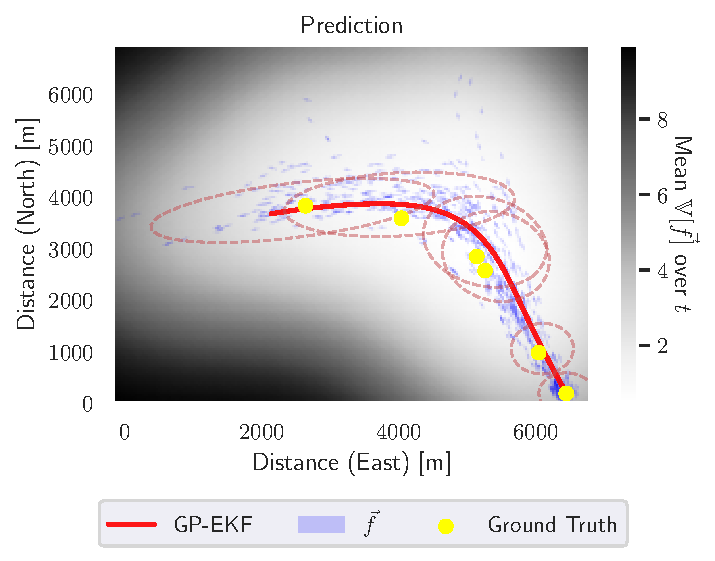
\includegraphics[width=\textwidth]{figures/dyngp/gp_ekf.pdf}
        \caption{Trajectory plotted against the vector-field $\vec{f}(\boldsymbol{x})$. The ellipses show the $95\%$ credibility interval for the predicted trajectory at the ground-truth timestamps.}
    \end{subfigure}
    \begin{subfigure}{\textwidth}
        \centering
        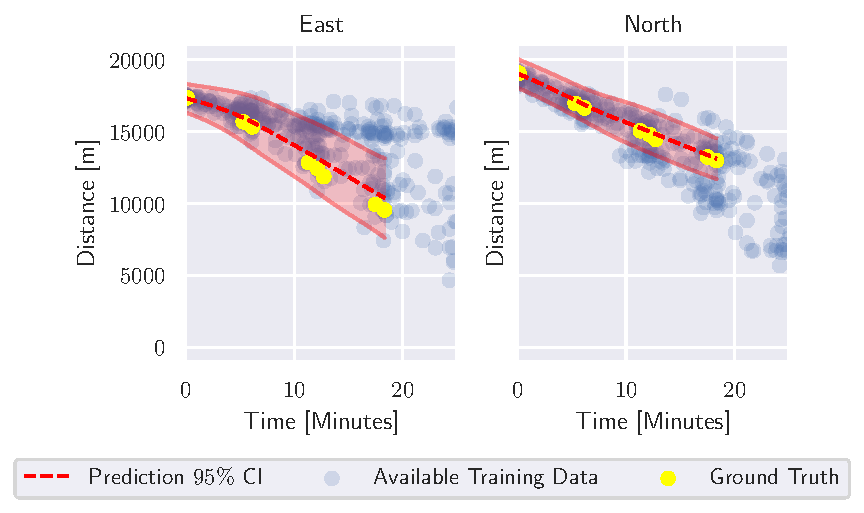
\includegraphics[width=\textwidth]{figures/dyngp/gp_ekf_state.pdf}
        \caption{$95\%$ credibility interval for the trajectory plotted against time}
    \end{subfigure}
    \caption{Predicted position using GP-EKF}
    \label{fig:gp_ekf}
\end{figure}



\section{Incorporating vessel position}
While the prediction procedure proposed in \cref{alg:gp_ekf_prediction} yields good predictions in many cases, it is inherently an open-loop prediction. Inaccurate predictions will never be corrected, propagating through any remaining iterations, potentially leading to significant errors later on. \todo[]{Add figure to showcase this issue} It would be desirable if the prediction converged towards available position measurements, \textit{slowly and only if the prediction is clearly wrong}. In other words, weak feedback compensating for minor prediction errors. Expressed using Bayes law
\begin{equation}\label{eq:gp_ekf_update_posterior}
    p(\boldsymbol{x}_{0:t} | \mathcal{D}) = \frac{p(\mathcal{D} | \boldsymbol{x}_{0:t}) p(\boldsymbol{x}_{0:t})}{p(\mathcal{D})} \propto p(\mathcal{D} | \boldsymbol{x}_{0:t})p(\boldsymbol{x}_{0:t})
\end{equation}
where $\mathcal{D}$ here is all available training data.

The problem is that the dataset $\mathcal{D}$ does not contain any samples from the target vessel's future trajectory, though it contains a lot of data from trajectories that are assumed to be similar. Thus, the challenge is to relate the target vessel's trajectory to the data-generating process for the dataset $\mathcal{D}$.

This is still very much considered an unsolved problem. This thesis attempts two different approaches, but the solutions are not yet satisfactory.

\subsection{Synthetic Likelihood}
This section is inspired by the work of \citeauthor{praveen-syn} \cite{praveen-syn}.

A proper likelihood $p(\mathcal{D} | \boldsymbol{x}_{0:t})$ is unavailable, or at least considered infeasible to compute. This motivates the use of so-called \textit{likelihood-free} methods, where the most common method is the \textit{Approximate Bayesian Computation} (ABC). Likelihood-free methods are used when the likelihood cannot be computed, while simulation from the model is still possible \cite{likelihood_free,frazier2021bayesian}. In this thesis, the focus will be on another likelihood-free approach, namely, the \textit{\acrfull{sl}} which replaces the likelihood by one or several approximate Gaussian summary statistics, $S_{0:t} = S(\boldsymbol{x}_{0:t}) \sim \mathcal{N}(\boldsymbol{\mu}(\boldsymbol{x}_{0:t}), \boldsymbol{\Sigma}(\boldsymbol{x}_{0:t}))$, of the data. Assuming the summary statistic contains sufficient information about $\boldsymbol{x}_{0:t}$, it should yield a good approximation of the true likelihood, i.e.
\begin{equation}
    p(\mathcal{D} | \boldsymbol{x}_{0:t}) \approx p(S_{0:t} | \boldsymbol{x}_{0:t})
\end{equation}

In this thesis, the likelihood is assumed to factorize into
\begin{equation}
    p(S_{0:T} | \boldsymbol{x}_{0:T}) = \prod_{t=0}^{T} p(S_t | \boldsymbol{x}_t)
\end{equation} and the summary statistic $S_i$ is selected as the mean of the samples in the vicinity of $\boldsymbol{x}_i$. A simple solution is to define the vicinity as a fixed radius around the state $\boldsymbol{x}_i$

\begin{equation}
    \mathcal{Y}_t = \mathcal{Y}_t(\boldsymbol{x}_t) = \{\boldsymbol{z}_i \in \mathcal{D} : \; ||\boldsymbol{x}_t - \boldsymbol{z}_i|| \leq r\}
\end{equation}
where the threshold $r$ is a fixed parameter. The summary statistic $S_i$ is then given by

\begin{equation}
    S_t = S(\boldsymbol{x}_t) = \frac{1}{N} \sum_{\boldsymbol{z}_i \in \mathcal{Y}_t} \boldsymbol{z}_i
\end{equation}
where $N$ is the number of samples in $\mathcal{Y}_t$. Assuming the measurements in $\mathcal{Y}$ are \acrshort{iid}, then the summary statistics is approximately Gaussian by the central limit theorem (see \cref{sec:clt}). By further assuming a simple measurement model
\begin{equation}\label{eq:gp_ekf_sl_z}
    \boldsymbol{z} = \boldsymbol{x} + \epsilon, \quad \epsilon \sim \mathcal{N}(0, \boldsymbol{R})
\end{equation}

yields the following distribution for the summary statistic given the predicted state $\boldsymbol{x}_i$

\begin{equation}
    p(S_t \;| \; \boldsymbol{x}_t) = \mathcal{N}(\boldsymbol{x}_t, \frac{\boldsymbol{R}}{N})
\end{equation}

The posterior distribution of the trajectory prediction can then be approximated by

\begin{align}\label{eq:gp_ekf_sl_approx_posterior}
    \begin{split}
        p(\boldsymbol{x}_{0:t} | \mathcal{D}) \approx p(\boldsymbol{x}_{0:t} | S_{0:t}) &= \frac{p(S_{0:t} | \boldsymbol{x}_{0:t}) p(\boldsymbol{x}_{0:t})}{p(S_{0:t})}\\
        &= \frac{p(S_t | \boldsymbol{x}_t)p(\boldsymbol{x}_t | \boldsymbol{x}_{t-1}) p(\boldsymbol{x}_{0:t-1} | S_{0:t-1})}{p(S_t | S_{0:t-1})}
    \end{split}
\end{align}
where the second equality yields a recursive formulation for the posterior distribution. As all distributions are Gaussian, \cref{eq:gp_ekf_sl_approx_posterior} boils down to the normal Kalman update step, using the summary statistic $S_i$ as measurement for each timestep.

The derivations in this section blindly make quite substantial assumptions that can seriously impact the results.
\begin{enumerate}
    \item The derivations claim the summary statistics are approximate Gaussian by the central limit theorem. The underlying assumption is that the data is \acrshort{iid} and that there is a large number of samples. As the samples originate from several types of vessels and from different trajectories, there is reason to suspect the samples might not be \acrshort{iid}.
    \item The measurement model in \cref{eq:gp_ekf_sl_z} assumes the measurements are distributed around the target vessel's trajectory. In practice, the samples might be heavily influenced by several different trajectories at once. This makes tuning $\boldsymbol{R}$ a challenge.
\end{enumerate}


\begin{figure}
    \centering
    \begin{subfigure}{\textwidth}
        \centering
        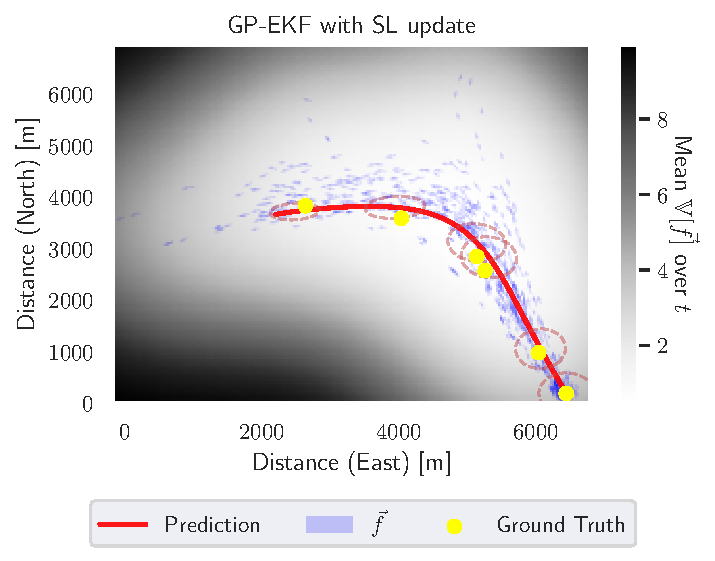
\includegraphics[width=\textwidth]{figures/dyngp/gp_ekf_with_syn.pdf}
        \caption{Trajectory plotted against the vector-field $\vec{f}(\boldsymbol{x})$. The ellipses show the $95\%$ credibility interval for the predicted trajectory at the ground-truth timestamps.}
    \end{subfigure}
    \begin{subfigure}{\textwidth}
        \centering
        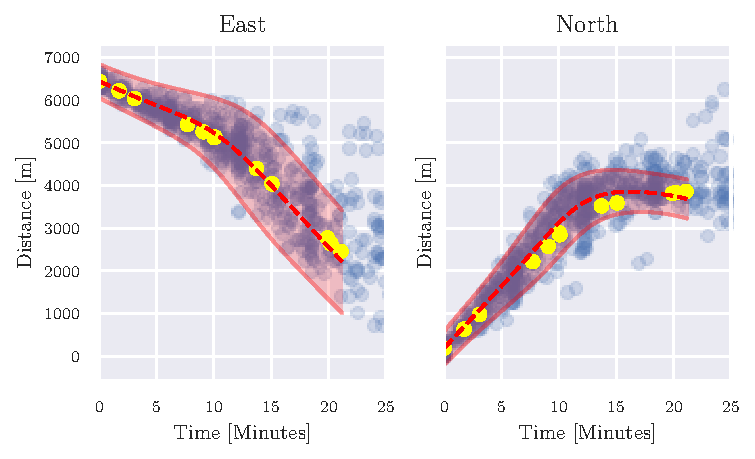
\includegraphics[width=\textwidth]{figures/dyngp/gp_ekf_with_syn_state.pdf}
        \caption{$95\%$ credibility interval for the trajectory plotted against time}
    \end{subfigure}
    \caption{Predicted position with the \acrshort{sl} update procedure.}
    \label{fig:gp_ekf_with_syn}
\end{figure}


\subsection{Probabilistic Data Association Filter}
The \acrshort{sl} update above ends up using an overly simplistic measurement model and does not consider the possibility that some measurements may originate from different underlying trajectories. For the target vessel following a specific underlying trajectory, the dataset may actually contain substantial false measurements which negatively affect the prediction. As the \acrshort{sl} update has no notion of false measurements, the result is overconfident uncertainty measurements can be seen in \cref{fig:gp_ekf_with_syn}.

This section attempts a rather different approach by incorporating the notion of data association into the mix. More specifically, the idea is to view the entire problem as single-target tracking and then apply the \textit{\acrfull{pdaf}} to solve the problem.

The \acrshort{pdaf} is a method commonly used in target tracking which combines data association and filtering. The following introduction to \acrshort{pdaf} is mostly inspired by \cite{sensorfusjon}, with some adaptations to fit the current problem better. As single target tracking and data association is not the topic of this thesis, only a short introduction to the \acrshort{pdaf} will be included here. For more details, see \cite{sensorfusjon,bar1995multitarget}

In this section, all measurements in the available training set are considered as \textit{virtual} \footnote{Virtual meaning a measurement that did not originate from the target vessel, but rather a measurement that could potentially originate from the target in the future. The word measurement is still used to keep the terminology similar to what is used by \acrshort{pdaf}.} position measurements, which may or may not originate from the vessel at time $t$. It is assumed \textbf{at most one} measurement may originate from the target to reduce the computational complexity significantly \cite{sensorfusjon}. The rest of the measurements are assumed to be clutter.

Given the predicted state $\hat{\boldsymbol{x}}_t$, any real measurement is expected to be distributed around this state due to some measurement noise. Following the notation used by \acrshort{ekf}, and using the measurement model $h(\boldsymbol{x}) = \boldsymbol{x} \implies H = \frac{\partial h (\boldsymbol{x})}{\partial \boldsymbol{x}} = I$, the predicted measurement distribution is expressed as in \cref{eq:gp_ekf_pdaf_measurement} where the innovation covariance is defined as $\boldsymbol{S}_t \triangleq \hat{\boldsymbol{P}}_t + \boldsymbol{R}$ and $\boldsymbol{R}$ is the measurement noise.

\begin{equation} \label{eq:gp_ekf_pdaf_measurement}
    \hat{\boldsymbol{z}}_t \sim \mathcal{N}(\hat{\boldsymbol{x}}_t, \boldsymbol{S}_{t}) = \mathcal{N}(\hat{\boldsymbol{x}}_t, \hat{\boldsymbol{P}}_t + \boldsymbol{R})
\end{equation}

There is also the possibility that none of the measurements originated from the target, and all observations are clutter. A good clutter model is a complicated topic, but the Poisson clutter model is used in this thesis. As the measurements are not actual measurements from the target, it is difficult to assign meaning to any clutter model. It, therefore, simply boils down to which parameters need to be tuned \footnote{The trajectory prediction is here considered to be target tracking of future position. The clutter parameters, therefore, need to be interpreted in the context of target tracking, not trajectory prediction.} and the Poisson clutter model should already be familiar to anyone with experience in target tracking.
Using the Poisson clutter model, the association probabilities are given by \cref{eq:pdaf_clutter_association_prob} \cite{sensorfusjon}, where $a_t$ is a discrete variable following a Categorical distribution where $a_t=k > 0$ denotes that measurement $k$ originated from the target. $a_t = 0$ is the special case when none of the measurements originated from the target, i.e., the predicted state should not be updated. $Z$ denotes a matrix of all the measurements (positions) available in the training data and is independent of time, i.e., all measurements are always potential candidates. $\lambda$ denotes the clutter rate, and $P_D$ denotes the probability of detecting the target vessel.
\begin{equation}\label{eq:pdaf_clutter_association_prob}
    \Pr\{a_t | Z\} \propto \begin{cases}
        \lambda (1 - P_D)                                                                 & a_t = 0 \\
        P_D \mathcal{N} (\boldsymbol{z}^{a_t} | \hat{\boldsymbol{x}}_t, \boldsymbol{S}_t) & a_t > 0 \\
    \end{cases}
\end{equation}

Using the likelihood for each of the possible outcomes, the association probabilities $\boldsymbol{\beta}$ can be computed by normalizing the likelihood, i.e.

\begin{equation}
    \beta_t^{a_t=i} = \frac{\Pr\{a_t=i \; | \; Z\}}{\sum_{k=0}^M \Pr\{a_t=k \; | \; Z\}}
\end{equation}

The predicted state can then by updated using the Kalman update procedure for each the measurements individually. As the measurements $\boldsymbol{z}_t^{a_t > 0}$ are known values, the state innovation $\boldsymbol{v}_t^{a_t>0} \triangleq \boldsymbol{z}_t^{a_t>0} - \hat{\boldsymbol{z}}_t$ is distributed according to the measurement prediction $\hat{\boldsymbol{z}}_t$.

\begin{equation}
    \boldsymbol{v}_t^{a_t>0} \sim \mathcal{N}(\boldsymbol{z}_t^{a_t>0} - \hat{\boldsymbol{x}}_t, S_t)
\end{equation}
The updated state for each measurement is then given by the normal \acrshort{ekf} update step

\begin{subequations}
    \begin{align}
        \boldsymbol{x}_t^{a_t > 0} & = \hat{\boldsymbol{x}}_t + \boldsymbol{W}_t \boldsymbol{v}_t^{a_t > 0} \\
        \boldsymbol{P}_t^{a_t > 0} & = \ (\boldsymbol{I} - \boldsymbol{W}_t) \hat{\boldsymbol{P}}_t
    \end{align}
\end{subequations}
where $\boldsymbol{W}_t \triangleq \hat{\boldsymbol{P}}_t \boldsymbol{S}_t^{-1}$ is the Kalman gain.
The updated state of the vessel over all possible measurements can be described as a Gaussian Mixture Model over the $M+1$ different modes weighted by the association probabilites, i.e.
\begin{equation}
    p(\boldsymbol{x_t}) = \underbrace{\beta_t^{a_t=0} \mathcal{N}(\boldsymbol{x}_t \; | \; \hat{\boldsymbol{x}}_t, \hat{\boldsymbol{P}}_t)}_{\text{No measurements are valid}} + \sum_{k=1}^M \underbrace{\beta_t^{a_t=k} \mathcal{N}\big(\boldsymbol{x}_t | \boldsymbol{x}_t^{a_t=k}, \boldsymbol{P}_t^{a_t=k}\big)}_{\text{Measurement $k$ is valid}}
\end{equation}


Moment reduction is then used to combined the different hypothesises into a single unimodal Gaussian distribution, i.e. a Gaussian distribution is fitted to the first and second moment (mean and variance) of the Gaussian mixture. The mean and variance of the resulting distribution is given by \cref{eq:pdaf_moment_mean} and \cref{eq:pdaf_moment_var} respectively, using $\boldsymbol{v}_t \triangleq \sum_{a_t > 0} \beta_t^{a_t} \boldsymbol{v}_t^{a_t}$.

\begin{subequations}
    \begin{align}
        \boldsymbol{x}_t & = \hat{\boldsymbol{x}}_t + \boldsymbol{W}_t \boldsymbol{v}_t \label{eq:pdaf_moment_mean} \\
        \begin{split}
            \boldsymbol{P}_t &= \hat{\boldsymbol{P}}_t - (1 - \beta_t^{0}) \boldsymbol{W}_t \boldsymbol{S}_t  \boldsymbol{W}_t\\ &+ \underbrace{\boldsymbol{W}_t \big[\sum_{a_t > 0}^M \beta_t^{a_t} \boldsymbol{v}_t^{a_t} (\boldsymbol{v}_t^{a_t})^\intercal - \boldsymbol{v}_t \boldsymbol{v}_t^\intercal \big] \boldsymbol{W}_t^\intercal}_{\text{spread of innovation}}\label{eq:pdaf_moment_var}
        \end{split}
    \end{align}
\end{subequations}

While available measurement could be used at each timestep, it is in practice more convenient only to include a subset that is close enough to the predicted state. As this measurement \textit{gate} should scale with the uncertainty, the gated subset is selected as \cref{eq:pdaf_gate} where $g$ is the number of standard deviations the method should consider.

\begin{equation} \label{eq:pdaf_gate}
    \mathcal{G} = \big\{ \boldsymbol{z}^{a_t > 0} \; | \; (\boldsymbol{z}^{a_t > 0} - \hat{\boldsymbol{x}}_t)^\intercal S^{-1} (\boldsymbol{z}^{a_t > 0} - \hat{\boldsymbol{x}}_t) < g^2 \big\}
\end{equation}


By combining the \acrshort{pdaf} update with the GP-EKF prediction procedure in \cref{alg:gp_ekf_prediction}, the predicted trajectory can be tuned to favor areas with a large number of samples, effectively pulling the state towards areas with available samples. Conversely, in regions with samples spread evenly around the predicted state, then the \acrshort{pdaf}'s effect is negligible (assuming proper tuning). 

\begin{algorithm}[h]
    \begin{algorithmic}[1]
        \Procedure{GP-EKF-PDAF}{$\hat{\boldsymbol{x}}_{t}$, $\hat{\boldsymbol{P}}_{t}$, | $\mathbf{R}$, $\lambda$, $p_D$, $g$}
        \State $\boldsymbol{S}_t = \hat{\boldsymbol{P}}_t + \boldsymbol{R}$ \Comment{Innovation Covariance}
        \State $\boldsymbol{W}_t = \hat{\boldsymbol{P}}_t \boldsymbol{S}_t^{-1}$\Comment{Kalman Gain}
        \For{each measurement $\boldsymbol{z}^{a_t > 0}$}
        \State $\boldsymbol{v}_t^{a_t>0} = \boldsymbol{z}^{a_t>0} - \hat{\boldsymbol{x}}_t$ \Comment{Innovation}
        \State $\tilde{\beta}^{a_t>0} = \mathcal{N}(\boldsymbol{v}_t^{a_t > 0} \; | \; 0, \boldsymbol{S}_t)$ \Comment{Unnormalized Weight}
        \EndFor
        \State $\tilde{\beta}_t^{a_t = 0} = \lambda (1-p_D)$ \Comment{Unnormalized Clutter Probability}
        \State $\boldsymbol{\beta} = \frac{\tilde{\boldsymbol{\beta}}}{\sum_{a_t} \tilde{\beta}^{a_t}}$ \Comment{Normalize weights}
        \State $\boldsymbol{v}_t = \sum_{a_t > 0} \beta^{a_t} \boldsymbol{v}_t^{a_t}$
        \State $\boldsymbol{x}_t = \hat{\boldsymbol{x}}_t + \boldsymbol{W}_t \boldsymbol{v}_t$\Comment{Update the state mean}
        \State $\tilde{\boldsymbol{P}}_t = \boldsymbol{W}_t \big[\sum_{a_t > 0}^M \beta_t^{a_t} \boldsymbol{v}_t^{a_t} (\boldsymbol{v}_t^{a_t})^\intercal - \boldsymbol{v}_t \boldsymbol{v}_t^\intercal \big] \boldsymbol{W}_t^\intercal$\Comment{Spread of innovation}
        \State $\boldsymbol{P}_t = \hat{\boldsymbol{P}}_t - (1 - \beta_t^{0}) \boldsymbol{W}_t \boldsymbol{S}_t  \boldsymbol{W}_t + \tilde{\boldsymbol{P}}_t$ \Comment{Updated state uncertianty}


        \State \textbf{return} $\boldsymbol{x}_t, \; \boldsymbol{P}_t$
        \EndProcedure
    \end{algorithmic}
    \caption{GP-EKF-PDAF update}
    \label{alg:gp_ekf_pdaf}
\end{algorithm}


\begin{figure}
    \centering
    \begin{subfigure}{\textwidth}
        \centering
        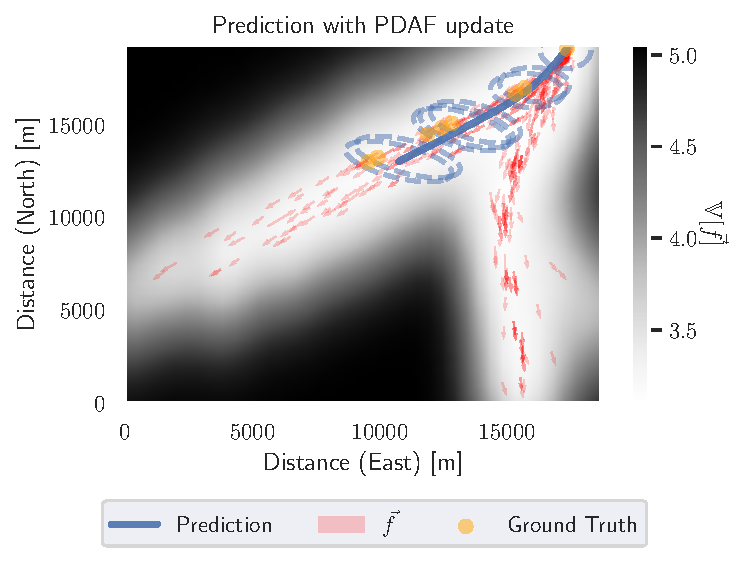
\includegraphics[width=\textwidth]{figures/dyngp/gp_ekf_with_pdaf.pdf}
        \caption{Trajectory plotted against the vector-field $\vec{f}(\boldsymbol{x})$. The ellipses show the $95\%$ credibility interval for the predicted trajectory at the ground-truth timestamps.}
    \end{subfigure}
    \begin{subfigure}{\textwidth}
        \centering
        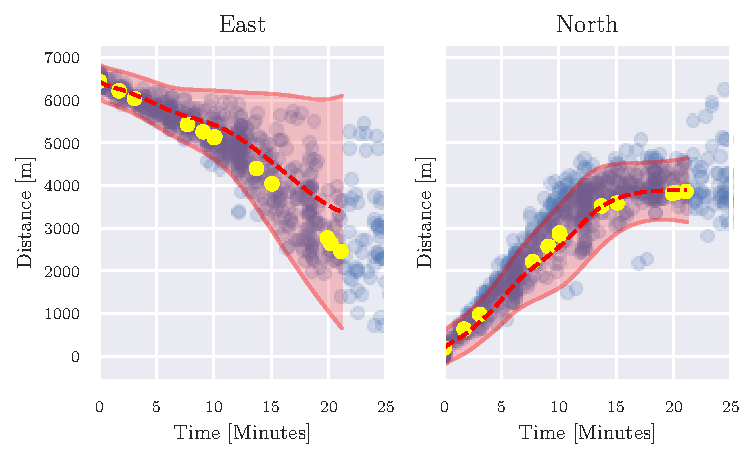
\includegraphics[width=\textwidth]{figures/dyngp/gp_ekf_with_pdaf_state.pdf}
        \caption{$95\%$ credibility interval for the trajectory plotted against time}
    \end{subfigure}
    \caption{Predicted position with the PDAF update procedure.}
    \label{fig:gp_ekf_with_pdaf}
\end{figure}

\subsubsection{Tuning PDAF parameters}
The model should primarily trust the prediction model, as it would get stuck as the measurements do not change over time. If the \acrshort{pdaf} parameters are tuned too aggressively, it tends to affect the velocity estimates of the prediction negatively. In practice, it has worked well tuning the measurement noise $\boldsymbol{R}$ to get the desired update effect.
However, finding a set of parameters that works well across different trajectories turns out to be challenging. Parameters that improve the prediction for one trajectory may do more harm than good on another. The performance of using PDAF will be explored further in \cref{chap:stat_testing}.

% \subsection{The ad-hoc approach}\todo[]{Consider removing}
% Neither the \acrshort{sl} nor the \acrshort{pdaf} approach is a satisfactory solution as both either have a negligible effect or suffers from overconfident uncertainty predictions. The problem lies in the assumptions that the observed positions originate from the target vessel, while in reality, the measurements are from entirely different trajectories. As long as the predicted state is in a densely populated area, the update steps will have no problem finding evidence supporting the current state, leading to overconfidence. Though not covered in this thesis, this problem motivates research into more sophisticated likelihood functions.

% During tuning both these methods, it became apparent that the desired behavior of these update steps would correct the prediction's mean and keep roughly the same level of uncertainty. In other words, the model should use the additional information from the update step to correct its prediction without reducing the uncertainty. While certainly not elegant, the quick and dirty solution was to omit the update of the state uncertainty, i.e., $\boldsymbol{P}_t = \hat{\boldsymbol{P}}_t$. This ad-hoc solution will be denoted the \textit{modified \acrshort{pdaf}} and the \textit{modified \acrshort{sl}} and works surprisingly well in practice. It is, however, not considered a good replacement for a proper likelihood.

\subsection{Simulating trajectories using Gaussian Process Sequential Monte Carlo}\label{sec:dyngp_particle}
The Kalman-based prediction scheme proposed in the previous section works well as long as a single Gaussian distribution can sufficiently explain the uncertainty. However, in branching trajectories, minor differences in position early in the predicted trajectory might significantly affect the following predictions. The result is a multimodal trajectory distribution, which a Kalman-based approach is not able to express.

Inspired by the prediction step used by \textit{particle filters} \cite{sensorfusjon}, the idea of sampling trajectories can be used to explore the multimodal trajectory distribution. While inspired by the particle filter, this approach will from now on be referred to as \textit{Sequential Monte-Carlo} to avoid confusion\footnote{a vital part of the particle filter is weighting the particles based on available measurements. As only the sampling of trajectories is performed, Sequential Monte-Carlo seems like a better fit.}, as well as to follow the same naming convention as used by \citeauthor{pedestrian} \cite{pedestrian}.

The derivation of the Sequential Monte-Carlo approach is embarrassingly simple as this method trades high computational complexity for more straightforward mathematics. Instead of analytical propagation of uncertainty, many trajectories are simulated through random sampling and used to express the uncertainty empirically. As a result, the uncertainty for any trajectory distribution can be described, though at the cost of considerable computational complexity.
$N$ different trajectories are initialized with similar initial conditions. The trajectories are then simulated by drawing independent increments from $\vec{f}$ using the approach described in \cref{sec:gp_samples}, conditioned on the current state of each trajectory. The result is visualized in \cref{fig:gp_particle} for $N=500$ trajectories.
\begin{figure}[h]
    \centering
    %\begin{subfigure}{\textwidth}
    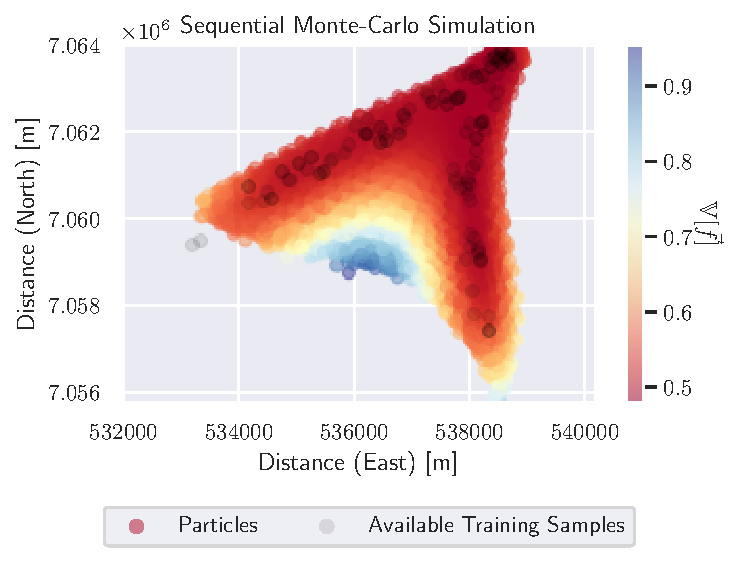
\includegraphics[width=\textwidth]{figures/dyngp/gp_particle.pdf}
    \caption{Trajectories simulated by sampling from $\vec{f}$. Notice how it is able to represent the multimodal trajectory distribution. }
    %\end{subfigure}
    %\begin{subfigure}{\textwidth}
    %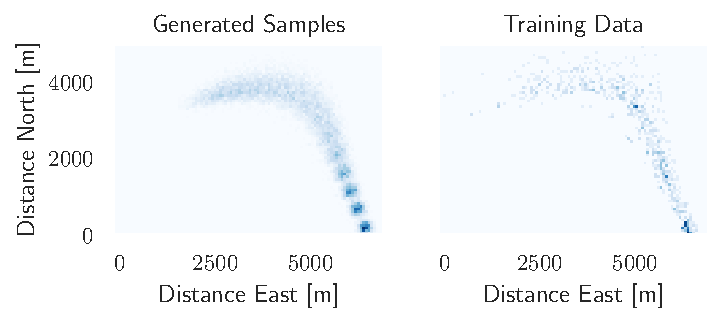
\includegraphics[width=\textwidth]{figures/gp_particle_hist.pdf}
    %\caption{}
    %\end{subfigure}
    \label{fig:gp_particle}
\end{figure}

\subsection{Training Source}
There are two potential sources for the training samples $\boldsymbol{y}$:

\begin{enumerate}
    \item Trajectories from the dataset are converted into training samples for $\vec{f}$ using the simple first-order finite-difference method in \cref{eq:finite_difference} between subsequent \acrshort{ais} samples in a trajectory $i$. This yields the training outputs $\boldsymbol{y}_t^{i}$ corresponding to the inputs $\boldsymbol{\eta}_t^i$ such that $\boldsymbol{y}_t^i = \vec{f}(\boldsymbol{\eta}_t^i) + \epsilon$.
    \item The \acrshort{cog} and \acrshort{cog} from the \acrshort{ais} data can be used directly.
\end{enumerate}

\begin{align}\label{eq:finite_difference}
    \boldsymbol{y}_t = \frac{\boldsymbol{x}_{t+1} - \boldsymbol{x}_t}{\tau_{t+1} - \tau_t}
\end{align}

A concern with using the \acrshort{cog} and \acrshort{sog} from the \acrshort{ais} is that this assumes the vessel's own estimates are accurate. The effect of this design choice is investigated further in \cref{chap:stat_testing}.


\section{Choice of kernel}
The approximation used to calculate the posterior distribution in \cref{eq:dyngp_true_posterior} is only a first-order Taylor approximation. Hence, it is only a reasonable approximation for functions with a low degree of nonlinearity, and care should be taken when designing the \acrshort{gp} dynamics $\vec{f}$. In this thesis, it is argued that \acrshort{rbf} kernel is the preferred choice due to the highly smooth characteristic of the functions drawn from this kernel. The \acrshort{rbf} kernel

\begin{equation}\label{eq:dyngp_kernel}
    k(\boldsymbol{\eta}, \boldsymbol{\eta}') = \sigma^2 \exp \big[ - \frac{1}{2} (\boldsymbol{\eta} - \boldsymbol{\eta}')^\intercal \boldsymbol{W}^{-1} (\boldsymbol{\eta} - \boldsymbol{\eta}')^\intercal\big]
\end{equation}
is found to work well in most cases, as long as the vessel follows a reasonably smooth trajectory. $\boldsymbol{W}$ is a diagonal matrix a separate lengthscale for each input dimension. The \acrshort{rbf} is the go-to kernel for the GP-EKF in this thesis, though other kernels, such as the Matern class of kernels, may work just as well, if not better.

The derivative of this kernel with respect to the $i$-th input dimension $\boldsymbol{\eta}[i]$ can be computed as \cite{pedestrian, gpekf}

\begin{equation}
    \frac{\partial k(\boldsymbol{\eta}, \boldsymbol{\eta}')}{\partial \boldsymbol{\eta}[i]} = -W_{ii}^{-1}(\boldsymbol{\eta}[i] - \boldsymbol{\eta}'[i]) \sigma^2 \exp \big[ - \frac{1}{2} (\boldsymbol{\eta} - \boldsymbol{\eta}')^\intercal \boldsymbol{W}^{-1} (\boldsymbol{\eta} - \boldsymbol{\eta}')^\intercal\big]
\end{equation}


A possible extension is to use the sum of two \acrshort{rbf} kernels to get some additional flexibility while still having a reasonably smooth function. This is the same kernel proposed in \cref{chap:direct_gp}, though without the \acrshort{cog} and \acrshort{sog} input dimensions. It works better than the \acrshort{rbf} kernel in some of the more complicated cases, though at the cost of more hyperparameters to tune. In simple cases, hyperparameter optimization \textbf{typically} reduces the scale parameter of one of the \acrshort{rbf} kernels such that the dependent noise kernel $k_1$ has a negligible effect. It is important to stress the word "typically," as this kernel is also more prone to bad local optima during hyperparameter optimization due to the additional parameters \cite{rasmussen} and may end up overfitting. If the length scales become too small, the dynamics $\vec{f}$ is allowed to become highly non-linear, and small changes in the input $\boldsymbol{x}$ may have a large impact on the prediction. The Taylor approximation is not a reasonable approximation in these cases, and the result is unstable uncertainty estimates \footnote{This is typically seen in the uncertainty estimates as large steps at seemingly random time steps, where the uncertainty experience sudden jumps as some elements in the Jacobian become large.}. The key takeaway is that the more flexible kernels are also more prone to overfitting, and care should be taken during optimization to avoid unrealistic parameters.

Other kernels may be preferred if the posterior density in \cref{eq:dyngp_true_posterior} is evaluated using sampling-based methods, such as Sequential Monte-Carlo, as the Taylor approximation does not limit these methods.  However, it is not covered by this thesis.


\subsection{Optimizing the hyperparameters}
The hyperparameters can be optimized using the \acrshort{ml} approach discussed in \cref{sec:gp_mle}.

The whole dataset cannot be used to find the optimal hyperparameters due to the computational complexity. Two approaches are proposed to mitigate this issue:
\begin{enumerate}
    \item Fit the hyperparameter to many different subsets of the available training data and use the median values. The median is preferred over the mean values to avoid issues with outlier parameter estimates. This approach tends to find a set of hyperparameters that work well across a wide range of cases but may become too general for challenging scenarios.
    \item Rerun the hyperparameter optimization for each scenario. This approach tends to find the optimal parameters in each case. However, it is also error-prone as it is not guaranteed to find a global optimum, and it may cause overfitting.
\end{enumerate}

The first approach is likely the preferred choice in practical applications, as the hyperparameter optimization is prone to bad local optima, and the results should ideally be inspected before deployment to real-world applications. A possible extension is to find a global set of parameters for each distinct vessel type, assuming a vessel's behavior is somewhat consistent across the entire region.

\section{Summary}
This chapter has so far introduced a lot of new concepts so that it might be nice with a summary of the overall pipeline:

\begin{enumerate}
    \item Based on the target vessel's current state, such as position, \acrshort{cog} and \acrshort{sog}, trajectories with similar initial conditions is selected from the training set.
    \item Training inputs $\boldsymbol{\eta}$ and outputs $\boldsymbol{y}$ for $\vec{f}$ are generated from the training trajectories.
    \item The kernel hyperparameters are optimized using \acrshort{ml} to find the parameters which best explains the training data. This is either done once to find a global set of parameters or individually for each scenario.
    \item The training data and kernel can then used to get the conditional distribution for $\vec{f}$.
    \item The \acrshort{ekf} procedure in \cref{alg:gp_ekf_prediction} is called repeatedly, using the current state of the target vessel as initial conditions. At each step, the \acrshort{pdaf} update procedure can be used as well if desired. Sequential Monte-Carlo can alternatively be used to simulate multimodal trajectories.
\end{enumerate}

The only parameters which need manual tuning are the time increment $\Delta \tau$ and the initial covariance $\boldsymbol{P}_0$. All other parameters are learned from the data.

\chapter{Statistical Testing}\label{chap:stat_testing}
Inspired by \cite{hexeberg}, the performance of the proposed models will be compared on straight-line and curved trajectories independently. This comparison is intended to showcase the methods' ability to consistently predict reasonable trajectories and motivate further research into \acrshort{gp} based methods. However, the content of this chapter is not intended to showcase a perfect solution, and the methods are still heavily influenced by how the hyperparameters are selected, as well as any tuning parameters.

\section{Method}

The simulation will test the performance on a total of $700$ different test trajectories, where one half corresponds to straight-line trajectories and the remaining half consists of curved trajectories. Trajectories are selected from the dataset proposed in \cref{chap:ais}, and will have a total duration of between $15$ and $30$ minutes. The Direct GP and GP-EKF from \cref{chap:direct_gp} and \cref{chap:gp_ekf}, respectively, will be tested on the same scenarios as defined in \cref{chap:ais} and get access to the exact same training data.

Three different metrics -- trajectory error, path error and normalized estimation error squared -- will be used to compare the performance of the various methods.

\subsection{Trajectory Error}
The trajectory error is found by comparing the predicted mean position with the ground truth. As the predicted trajectory is simulated in discrete time, the points with the closest timestamps are used for comparison. The simulation will use $\Delta \tau = 10\text{ seconds}$, which yields a maximum error in time $\frac{\Delta \tau}{2} = 5 \text{ seconds}$, which is considered to be acceptable considering the time-horizon of between $15$ and $30$ minutes.
\subsection{Path Error}
The path error is defined as the closest point in the predicted trajectory to each point in the ground truth, under the constraint that the corresponding predicted timestamps must be monotonically increasing. In other words, the path cannot move backwards in time. Linear interpolation is used to get the path error at fixed timestamps to simplify the comparison.

\subsection{Normalized Estimation Error Squared}
For the uncertainty estimates to provide any value, the predictions must be consistent. In this context, the term consistency is borrowed from the term \textit{filter consistency} used when tuning Kalman filters \cite{sensorfusjon}. The idea is that prediction errors, on average, should scale with the state covariance. In other words, the model should not place much confidence in a prediction that is wrong while being highly confident when a prediction is correct. Consistency can also be interpreted using a frequentistic interpretation of probability, where after many predictions, the state uncertainty should reflect the actual error rate.

The \textit{\acrfull{nees}} is a metric that can be used to quantify consistency and is given by
\begin{equation}
    \text{NEES} = (\boldsymbol{x} - \hat{\boldsymbol{x}})^\intercal \boldsymbol{P}^{-1} (\boldsymbol{x} - \hat{\boldsymbol{x}})
\end{equation}

where $\boldsymbol{x}$ is ground truth and $\hat{\boldsymbol{x}}$ refers to the prediction.

Assuming that the prediction error follows a Gaussian distribution, the \acrshort{nees} follows a Chi-Squared distribution which can be used to form a confidence interval. Comparing the prediction errors with this confidence interval can then be used to get a sense of whether the estimated state uncertainty is consistent with the actual error rate.

\subsection{Comparing distributions - Boxplot}
The boxplot is used to visualize the distribution of the different metrics. The boxplot visualizes the estimated quartiles, i.e. the $25\%$, $50\%$, and $75\%$ quantiles, of the distribution. The "whiskers" show the range of values not considered to be outliers. Points outside of $[Q_{25} - 1.5 \text{ IQR}, Q_{75} + 1.5 \text{ IQR}]$ are considered outliers, where $\text{IQR} = Q_{75} - Q_{25}$ is the \text{inter-quartile range} \cite{matplotlib}.

\subsection{Interpolation}
The metrics will be compared at fixed $5$ minute intervals using linear interpolation. The error for short trajectories is not extrapolated, so there might be fewer available samples for the metrics when moving past $15$ minutes.

\subsection{Baseline - Constant Velocity Model}
As a basis of comparison, the \textit{\acrfull{cvm}} method is used as a baseline. The model uses the initial \acrshort{cog} and \acrshort{sog} to predict a straight line, where the vessel is assumed to keep a constant velocity and heading.

\subsection{Selecting test cases}
The two datasets from \cref{chap:ais} are used to perform the statistical testing.

However, $54\%$ of the dataset originates from only three ferries. Distinct discontinuities characterize the trajectories of these ferries as the vessels dock for short periods before moving back the same way they came. These discontinuities directly contradict the assumptions of smoothness made by the \acrshort{gp}s used in this thesis. Whether or not to include these vessels was a challenging decision, as a \acrshort{colav} will need to be able to handle ferries, just as any other vessel type. However, in a practical application, it is natural to distinguish between different vessel types and allow the use of more specialized models to handle cases such as frequently docking ferries. As no such distinction is made in this thesis, the statistical testing will be more insightful without using edge-cases for more than $50\%$ of the test cases. While it would be possible to not completely remove these vessels, i.e. perform subsampling, it is considered more confusing. Therefore, the samples from these three vessels are removed from the test set, though they are still present in the training set. This thesis has not proposed any method for filtering the training data based on the \acrshort{mmsi}; removing these vessels from the training set would be an unfair advantage.

The result is an artificial bias favoring the \acrshort{gp} framework proposed in this thesis, as the fraction of smooth trajectories has been artificially increased.

\subsubsection{Straigth-line trajectories}
The methods are first compared to the \acrshort{cvm} on simple straight-line trajectories. The statistics are based on $350$ randomly sampled trajectories without replacement that satisfy the following requirements:
\begin{enumerate}
    \item The sum of subsequent changes in \acrshort{cog} must be less than $30$ degrees, i.e. $\sum_i |(\mathcal{X}_{t+1} - \mathcal{X}_t)| \leq 30^\circ$. This requirement ensures a straight-line trajectory. Additional care is always taken to use the smallest possible difference as the angles $\mathcal{X} \in [0^\circ, 360^\circ)$ wraps around.
    \item There must be sufficient data available for training in the neighborhood around the initial starting point, with similar initial heading and speed. After sanitizing the dataset and removing irrelevant trajectories, at least $3$ trajectories need to be available for training.
    \item The overall duration of the trajectories must be between $15$ and $30$ minutes to be considered a test candidate.
\end{enumerate}

\subsubsection{Curved Trajectories}
The curved trajectory statistics are based on $350$ randomly sampled trajectories that satisfy the following requirements:
\begin{enumerate}
    \item The sum of subsequent changes in \acrshort{cog} must be greater than $40$ degrees, i.e. $\sum_i |(\mathcal{X}_{t+1} - \mathcal{X}_t)| \geq 40^\circ$. This requirement ensures a minimum curvature in the trajectory. Additional care is always taken to use the smallest possible difference as the angles $\mathcal{X} \in [0^\circ, 360^\circ)$ wraps around.
    \item There must be sufficient data available for training in the neighborhood around the initial starting point, with similar initial heading and speed. After sanitizing the dataset and removing irrelevant trajectories, at least $3$ trajectories need to be available for training.
    \item The overall duration of the trajectories must be between $15$ and $30$ minutes to be considered a test candidate.
\end{enumerate}

\subsection{Training Data}
The initial conditions for each test trajectory are considered a distinct scenario, and the relevant training data is selected according to the method proposed in \cref{chap:ais}. The requirements are restated here with the concrete values used for testing:

\begin{enumerate}
    \item The trajectories' initial position must be close to the target vessel's position $\boldsymbol{x}_0$. A fixed threshold at $||\Delta \boldsymbol{x}_0|| \leq 200 \text{ m}$ is used, where $\Delta \boldsymbol{x}_0$ is the difference between the target vessel's current position and the initial conditions of a potential training trajectory.
    \item The trajectories' initial \acrshort{cog} must be close to the target vessel's heading $\mathcal{X}$. A fixed threshold at $\mathcal{X} \pm 20^\circ$ is used, with additional care taken when the angles wrap.
    \item The trajectories' initial \acrshort{sog} must be close to the queried velocity $v$. A fixed threshold at $v \pm 4 \text{ knots}$ is used.
\end{enumerate}

Due to the way trajectories are generated from the \acrshort{ais} dataset, there will be significant overlaps between trajectories. Therefore, naively dividing the trajectories into a train and test set is considered insufficient, as sub-trajectories from the test set might also exist in the training set. Instead, the entire dataset is available for training, but all trajectories with identical MMSI and date as the test trajectory are removed before training. The date requirement ensures that trajectories for the same vessel can be used for training on any other day. There is still the possibility of leaking data from the test set if the trajectory moves past midnight, but this is assumed only to affect a negligible number of trajectories.


\section{Implementation}
The implementation details for each method are described in this section.

\subsection{Direct GP}
The excact \acrshort{gp} formulation is implemented using the \texttt{GaussianProcessRegressor} from the Python library, \textit{scikit-learn} \cite{scikit-learn}. The library supports all kernels introduced in \cref{chap:theory} and supports hyperparameter optimization using multiple restarts to avoid bad local optima.

The slightly more complicated kernel in \cref{eq:direct_gp_kernel} from \cref{chap:direct_gp} is used. This kernel is preferred over a single \acrshort{rbf} kernel as it simply yields the best performance across a range of different simulations. The noise term $\sigma^2$ is included as a White kernel and optimized like any other hyperparameter. The parameters are optimized for each test scenario, using $10$ random restarts to reduce the risk of bad local optima.

\subsection{GP-EKF}
The GP-EKF is tested with and without both the \acrshort{sl} and the \acrshort{pdaf} update steps, as well as using both finite difference and the \acrshort{cog}/\acrshort{sog} from the \acrshort{ais} dataset, resulting in $6$ different instances.

The GP-EKF requires more flexibility during development. Due to the need for calculating the gradient $\frac{\delta \vec{f}}{\delta \boldsymbol{x}}$, it is impractical to use existing \acrshort{gp} implementations. Due to the simple implementation of \cref{alg:gp_prediction}, it is easier to implement it from the ground up rather than adapting existing solutions.
The GP-EKF used in this thesis is therefore implemented directly in Python using only \textit{scipy}\cite{scipy} and \textit{numpy}\cite{numpy} to speed up linear algebra routines. The Cholesky decomposition in \cref{alg:gp_prediction} can be computed using \texttt{scipy.linalg.cho\_factor}, which calls a highly optimized LAPACK routine. Similarily, \texttt{scipy.linalg.solve\_\-trianglular} can be used to solve the lower triangular system of equations by forward substitution. The implementation of GP-EKF and the \acrshort{pdaf} update is then straightforward using \cref{alg:gp_ekf_prediction} and \cref{alg:gp_ekf_pdaf} from \cref{chap:gp_ekf}. The implementation used for the statistical testing use standardized training outputs $\boldsymbol{y}$.

For statistical testing, the proposed \acrshort{rbf} kernel from \cref{eq:dyngp_kernel} with independent length scales will be used due to its simplicity. More complicated kernels are avoided due to challenges with bad local optima during hyperparameter optimization.

The hyperparameters are tuned using the \acrshort{gp} implementation in the popular \textit{scikit-learn} \cite{scikit-learn} Python package. $10$ random restarts are used during optimization to reduce the risk of bad local minima. A lower bound constraint for the length scales is also used to avoid obvious overfitting and requires the length scales to be greater than $50$. Due to the wide variety of different scenarios on the training set, the hyperparameters are optimized for each iteration. This way, the robustness of the optimization is indirectly tested, as instances of bad local optima are included in the results.


The remaining parameters not found through \acrshort{ml} are tuned through trial and error on a few different trajectories.
The initial state uncertainty is set to $\boldsymbol{P}_0 = 500^2 \cdot \boldsymbol{I}$, which was found to work well during development. The \acrshort{pdaf} parameters are available in \cref{table:stats_pdaf_params} and the \acrshort{sl} parameters can be found in \cref{table:stats_sl_params}.

\begin{table}[h]
    \centering
    \begin{subtable}{0.49\textwidth}
        \begin{tabular}{|lll|}
            \textit{\textbf{Parameter}} &                                & \textit{\textbf{Value}}      \\ \hline
            Measurement noise           & $\boldsymbol{R}_{\text{PDAF}}$ & $500^2 \cdot \boldsymbol{I}$ \\
            Detection Probability       & $p_D$                          & $0.8$                        \\
            Clutter Rate                & $\lambda$                      & $2 \cdot 10^{-3}$            \\
            Gate Size                   & $g$                            & $2$
        \end{tabular}
        \caption{Parameters used for \acrshort{pdaf} update}
        \label{table:stats_pdaf_params}
    \end{subtable}
    \begin{subtable}{0.49 \textwidth}

        \centering
        \begin{tabular}{|lll|}
            \textit{\textbf{Parameter}} &                              & \textit{\textbf{Value}}      \\ \hline
            Noise                       & $\boldsymbol{R}_{\text{SL}}$ & $500^2 \cdot \boldsymbol{I}$ \\
            Search Radius               &                              & $50$                         \\
                                        &                              &                              \\
                                        &                              &
        \end{tabular}
        \caption{Parameters used for the SL update}
        \label{table:stats_sl_params}
    \end{subtable}
\end{table}



\section{Results}
The error metrics for straight-line and curved trajectories are available in \cref{table:stats_straight_line_error} and \cref{table:stats_curved_error} respectively, while the \acrshort{nees} results are available in \cref{table:stats_nees_straight} and \cref{table:stats_nees_curved}. All tables are found at the end of this chapter. Some hand-picked test scenarios are also included in \cref{chap:gp_ekf_examples} for the different GP-EKF variations.

This section will take a hierarchical approach, where the GP-EKF using finite-difference for training data is considered the basic configuration of the GP-EKF and will be used as a baseline when comparing the different variants of the GP-EKF. Unless explicitly stated otherwise, it is safe to assume that the GP-EKF uses finite-difference and no update step. For comparing specific combinations, the reader is referred to \cref{table:stats_straight_line_error} and \cref{table:stats_curved_error}.

As a base of comparison, the Direct GP and GP-EKF are compared to the \acrshort{cvm} on both straight-line and curved trajectories in \cref{fig:stats_both_vs_cvm}. On straight-line trajectories, both methods perform worse than the \acrshort{cvm} with higher trajectory error for all respective quartiles. As expected, the \acrshort{cvm} struggles on curved trajectories, whereas both the Direct GP and GP-EKF approaches perform significantly better with both lower median error and spread. The Direct GP approach performs slightly better than the GP-EKF, with lower median trajectory error and lower spread for both straight-line and curved trajectories. When comparing the path error for straight-line trajectories in \cref{table:stats_straight_path_err}, the GP-EKF performs consistently better than the Direct GP approach, with lower mean and median path error. The GP-EKF even outperforms the \acrshort{cvm} on straight-line paths when predicting beyond $15$ minutes.

Both the Direct GP and the GP-EKF approach perform better on curved trajectories as opposed to straight-line trajectories. After manually inspecting the test cases, it appears that many of the straight-line test cases belong to slow-moving vessels that are part of longer curved trajectories.  The training samples used to fit the \acrshort{gp}s in these cases often contain samples from faster-moving vessels, making the \acrshort{gp}s overshoot in their predictions. This hypothesis is corroborated by the path error in \cref{table:stats_straight_path_err}, as the GP-EKF outperforms the \acrshort{cvm} on long straight-line paths.

Neither the Direct GP nor the GP-EKF yield consistent uncertainty estimates as found by comparing the \acrshort{nees} to the theoretical $\mathcal{X}^2$ quartiles in \cref{fig:stats_straigth_nees_basic} and \cref{fig:stats_curved_nees_basic}. For both methods, the \acrshort{nees} is especially bad for straight-line trajectories with estimated quartiles exceeding the theoretical quartiles, which is likely linked to the increased error for the straight-line trajectories. The Direct GP approach performs better than the GP-EKF, with the $25\%$ and $50\%$ quartiles close to the theoretical values, while the basic GP-EKF remains overconfident for all quartiles. The upper quartile for both methods exceeds the theoretical value for the $\mathcal{X}^2$ distribution.

\subsection{GP-EKF: Finite Difference vs. COG/SOG from AIS}

\begin{figure}[h]
    \centering
    \makebox[\textwidth][c]{
        \begin{subfigure}{0.65\textwidth}
            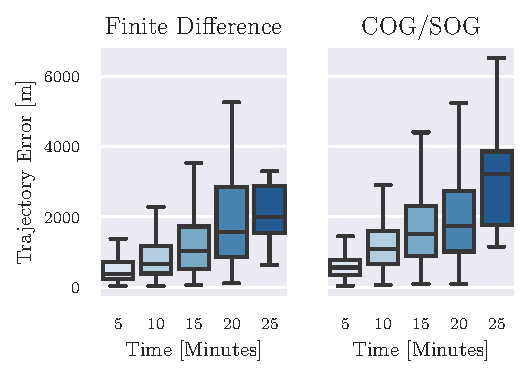
\includegraphics{figures/straight_line_stats/gp_cog_vs_fd.pdf}
            \caption{Straight-Line Trajectory}
        \end{subfigure}
        \begin{subfigure}{0.65\textwidth}
            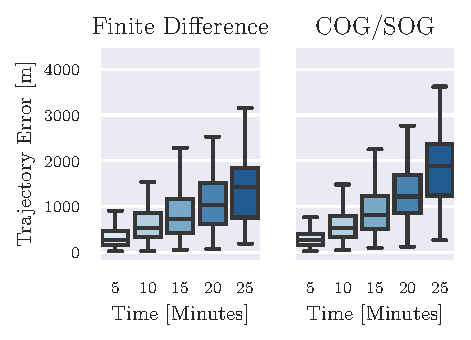
\includegraphics{figures/curved_line_stats/gp_cog_vs_fd.pdf}
            \caption{Curved Trajectory}
        \end{subfigure}
    }
    \caption{GP-EKF using finite differences and the \acrshort{cog} and \acrshort{sog} from the AIS dataset on $350$ trajectories. The finite difference approach performs slightly better, with lower median error and spread.}
    \label{fig:stats_gp_ekf_fd_vs_cog}
\end{figure}


A key design choice for the GP-EKF is deciding which data source to use for training. The model can either be trained using the \acrshort{cog} and \acrshort{sog} values contained in the \acrshort{ais} samples or by calculating numerical derivatives of the position through a finite-difference approach. \cref{fig:stats_gp_ekf_fd_vs_cog} compares the difference side-by-side. For straight-line trajectories, the results are remarkably similar. The finite difference approach seems to have a slight advantage on the lower quartile error at $\tau=25 \text{ minutes}$, though with an increased spread and the advantage is likely due to random errors. The finite difference performs slightly better than \acrshort{cog}/\acrshort{sog} for curved trajectories, especially as time increases, and has both lower median trajectory error and spread.

For the path errors in \cref{table:stats_straight_path_err} and \cref{table:stats_curved_path_err}, the results favor the \acrshort{cog}/\acrshort{sog} approach, with overall lower mean and median path errors when compared to the finite difference approach.

Using \acrshort{cog}/\acrshort{sog} yields a considerable \acrshort{nees} improvement over the finite difference approach, as seen in \cref{fig:stats_straigth_nees_cog_vs_fd} and \cref{fig:stats_curved_nees_cog_vs_df}. On curved trajectories, the estimated \acrshort{nees} quartiles are close to the theoretical values when using \acrshort{cog}/\acrshort{sog} as input data, while the finite difference approach yields overconfident results. A similar pattern is found for the median \acrshort{nees} values in \cref{table:stats_nees_straight} and \cref{table:stats_nees_curved} for all variants of the GP-EKF. 

\subsection{GP-EKF: Incorporating positions data}
The effect on the mean prediction for both the \acrshort{pdaf} and the \acrshort{sl} update procedures is compared to the basic GP-EKF configuration in \cref{fig:stats_gp_ekf_with_or_without_update}. The results are incredibly similar for both straight-line and curved trajectories. On closer inspection, there appears to be a slight advantage to using the \acrshort{pdaf} update step, but the improvement is within the margin of error, so it is not possible to draw any definitive conclusion.

However, the \acrshort{sl}, and to some extent the \acrshort{pdaf} update, have a detrimental effect on the \acrshort{nees}, leading to even more overconfident predictions. This is apparent when comparing the GP-EKF NEES with and without the update steps in \cref{fig:stats_straight_nees_update} and \cref{fig:stats_curved_nees_update}, as the \acrshort{nees} for the \acrshort{sl} update explodes compared to the basic GP-EKF method. Similar patterns are found in \cref{table:stats_nees_straight} and \cref{table:stats_nees_curved} regardless of whether the GP-EKF is trained with finite difference or \acrshort{cog}/\acrshort{sog} data.

\begin{figure}
    \centering
    \begin{subfigure}{\textwidth}
        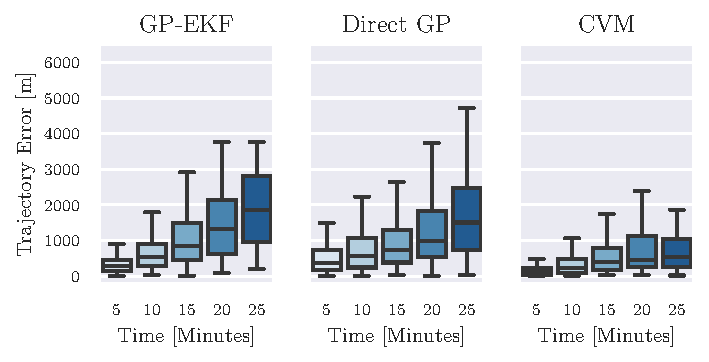
\includegraphics[width=\textwidth]{figures/straight_line_stats/both_vs_cvm.pdf}

        \caption{Straight-line trajectories.}
        \label{fig:stats_curved_both_vs_cvm}
    \end{subfigure}
    \begin{subfigure}{\textwidth}
        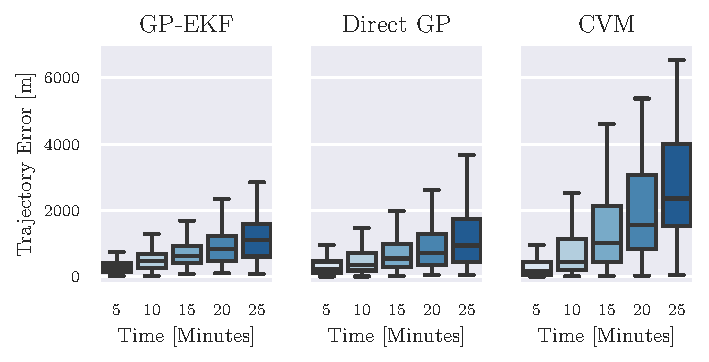
\includegraphics[width=\textwidth]{figures/curved_line_stats/both_vs_cvm.pdf}
        \caption{Curved trajectories.}
        \label{fig:stats_straight_both_vs_cvm}
    \end{subfigure}
    \caption{GP-EKF and Direct GP compared to a \acrshort{cvm} on $350$ straight-line and $350$ curved trajectories. For straight-line trajectories, the \acrshort{cvm} outperforms both the GP-EKF and the Direct GP, while the Direct GP yield slightly better performance than the GP-EKF. For curved trajectories, the \acrshort{cvm} struggles as expected. Both the GP-EKF and the Direct GP yields far better results with lower error and lower spread, while Direct GP has the lowest overall trajectory error quartiles. Interestingly, both GP-EKF and Direct GP performs better on curved trajectories than straight-line trajectories, with lower overall error and spread.}
    \label{fig:stats_both_vs_cvm}
\end{figure}



\begin{figure}[h]
    \centering
    \begin{subfigure}{1\textwidth}
        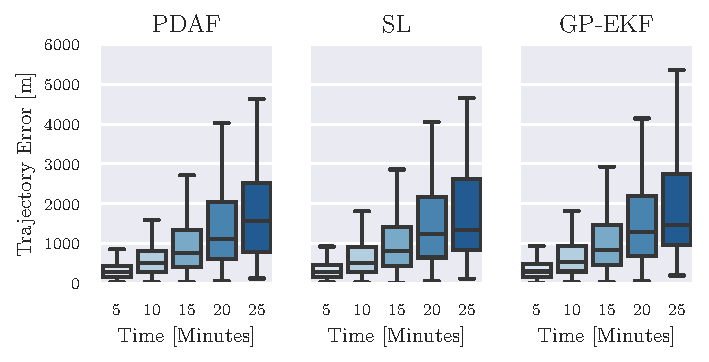
\includegraphics[width=\textwidth]{figures/straight_line_stats/gp_vs_update.pdf}
        \caption{Straight-Line Trajectories}
    \end{subfigure}
    \begin{subfigure}{1\textwidth}
        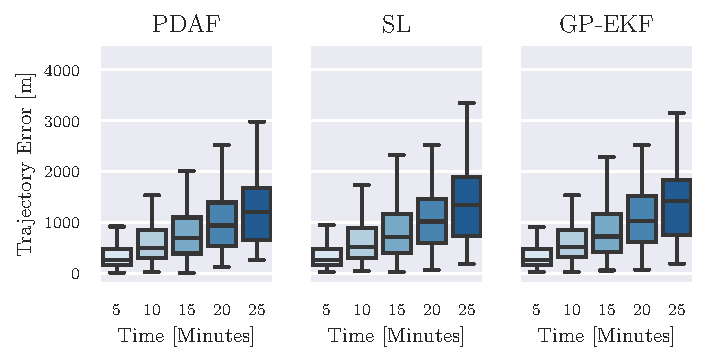
\includegraphics[width=\textwidth]{figures/curved_line_stats/gp_vs_update.pdf}
        \caption{Curved Trajectories}
    \end{subfigure}
    \caption{GP-EKF with and without the \acrshort{sl} and \acrshort{pdaf} updates on $350$ straight-line and $350$ curved trajectories. While there are some slight differences, the \acrshort{pdaf} and \acrshort{sl} update does not appear to have any considerable effect on the trajectory errors. On straight-line trajectories, the results are almost identical across all three variants. On curved trajectories, the \acrshort{pdaf} yields slightly lower error for the median and upper quartiles, though the difference is well within the margin of error.}
    \label{fig:stats_gp_ekf_with_or_without_update}
\end{figure}

% \begin{figure}[h]
%     \centering
%     \begin{subfigure}{1\textwidth}
%         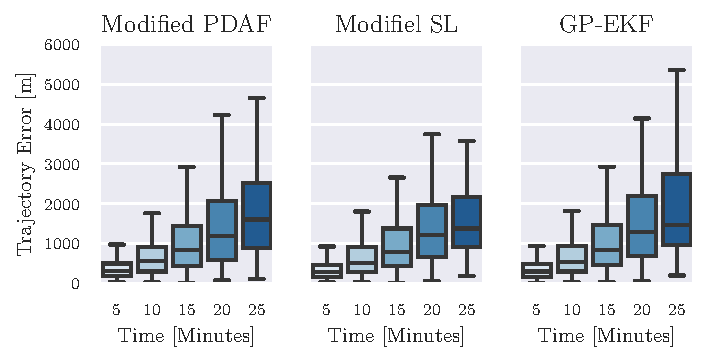
\includegraphics[width=\textwidth]{figures/straight_line_stats/gp_vs_update_no_P.pdf}
%         \caption{Straight-Line Trajectories}
%     \end{subfigure}
%     \begin{subfigure}{1\textwidth}
%         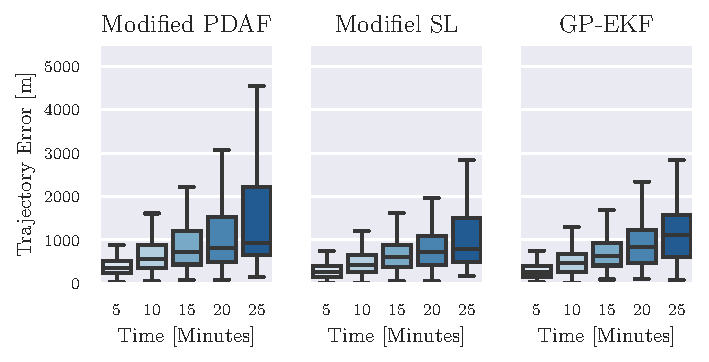
\includegraphics[width=\textwidth]{figures/curved_line_stats/gp_vs_update_no_P.pdf}
%         \caption{Curved Trajectories}
%     \end{subfigure}
%     \caption{GP-EKF with and without the modified \acrshort{sl} and \acrshort{pdaf} on curved trajectories for $350$ trajectories. The modified \acrshort{sl} performs better than the basic GP-EKF on straight-line trajectories for the upper $75\%$ quartile, while the modifed \acrshort{pdaf} performs about the same as the stock GP-EKF.  The modifed \acrshort{pdaf} performs worse than the basic GP-EKF on curved trajectories, while the modified \acrshort{sl} performs about the same.}
%     \label{fig:stats_gp_ekf_with_or_without_update_no_P}
% \end{figure}

\begin{figure}
    \centering
    \makebox[\textwidth][c]{
        \begin{subfigure}{0.6\textwidth}
            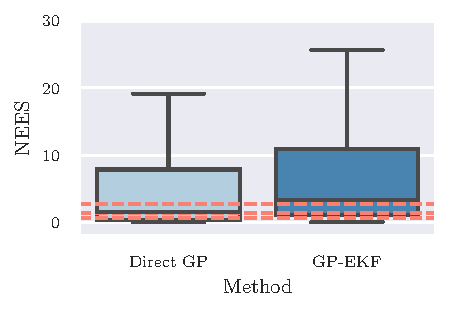
\includegraphics{figures/straight_line_stats/nees_vs_theoretical.pdf}
            \caption{Straight-Line Trajectory NEES Baseline}
            \label{fig:stats_straigth_nees_basic}
        \end{subfigure}
        \begin{subfigure}{0.6\textwidth}
            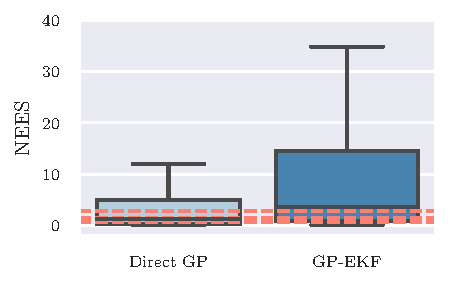
\includegraphics{figures/curved_line_stats/nees_vs_theoretical.pdf}
            \caption{Curved Trajectory NEES Baseline}
            \label{fig:stats_curved_nees_basic}
        \end{subfigure}
    }
    \makebox[\textwidth][c]{
        \begin{subfigure}{0.6\textwidth}
            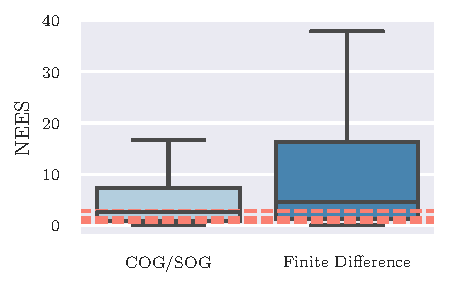
\includegraphics{figures/straight_line_stats/nees_vs_theoretical_cog_vs_fd.pdf}
            \caption{Straight-Line Trajectory COG/SOG vs Finite Difference}
            \label{fig:stats_straigth_nees_cog_vs_fd}
        \end{subfigure}
        \begin{subfigure}{0.6\textwidth}
            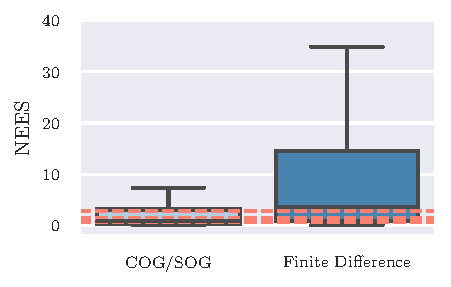
\includegraphics{figures/curved_line_stats/nees_vs_theoretical_cog_vs_fd.pdf}
            \caption{Curved Trajectory COG/SOG vs Finite Difference}
            \label{fig:stats_curved_nees_cog_vs_df}
        \end{subfigure}
    }
    \makebox[\textwidth][c]{
        \begin{subfigure}{0.6\textwidth}
            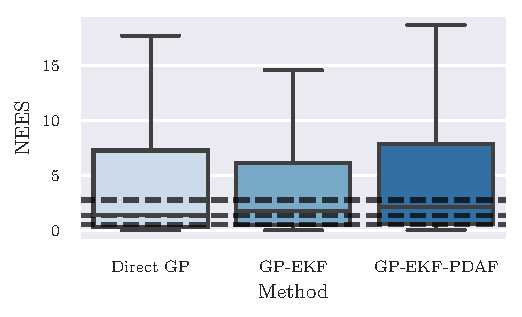
\includegraphics{figures/straight_line_stats/nees.pdf}
            \caption{Straight-Line Trajectory with update steps}
            \label{fig:stats_straight_nees_update}
        \end{subfigure}
        \begin{subfigure}{0.6\textwidth}
            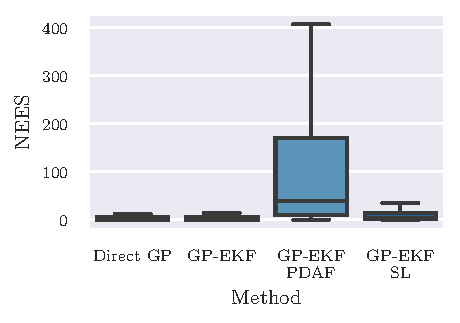
\includegraphics{figures/curved_line_stats/nees.pdf}
            \caption{Curved Trajectory with update steps}
            \label{fig:stats_curved_nees_update}
        \end{subfigure}
    }

    \caption{A comparison of the NEES for the different methods. The top row compares the \acrshort{nees} for the Direct GP and the base GP-EKF to the theoretical quartile values for the $\mathcal{X}^2$ distribution (red dashed lines) and is intended as a base of comparison. The second row compares the difference in consistency between using \acrshort{cog}/\acrshort{sog} and finite difference as input data. The last row compares the effect of the update steps for the GP-EKF. The theoretical quartiles are not included in the last row due to the large differences in scale, and the reader is advised to use the Direct GP and basic GP-EKF for comparison.}

\end{figure}

% On straight-line trajectories, the $25\%$ and $50\%$ quartiles correspond well with the theoretical values for the $\mathcal{X}^2$ distribution for all methods. The \acrshort{pdaf} update step does, however, reduce the predicted uncertainty, leading to increased overconfidence. In addition, the estimated \acrshort{nees} distribution has a much fatter right-tail than the theoretical $\mathcal{X}^2$ distribution, leading to an estimated $75\%$ quartile far outside the theoretical values.

% On curved trajectories, the GP-EKF with and without PDAF is consistently overconfident. The theoretical quartiles are not plotted due to the large y-axis. The direct \acrshort{gp} approach performs significantly better, which is why a separate plot in \cref{fig:stats_curved_nees_direct} is added to compare it to theoretical quartiles.




\begin{table}[b]
    \begin{subtable}{\textwidth}
        \makebox[\textwidth][c]{
            \begin{tabular}{lllrrrrr}
                \toprule
                        &                & Time [Minutes]    & 5   & 10  & 15   & 20   & 25   \\
                Summary & Method         & Training Source   &     &     &      &      &      \\
                \midrule
                Mean    & CVM            & COG/SOG from AIS  & 172 & 383 & 623  & 786  & 772  \\
                        & Direct GP      & Position          & 603 & 720 & 944  & 1269 & 1727 \\
                        & GP-EKF         & COG/SOG from AIS  & 328 & 668 & 1090 & 1560 & 2048 \\
                        &                & Finite Difference & 331 & 656 & 1029 & 1417 & 1917 \\
                        & GP-EKF w/ PDAF & COG/SOG from AIS  & 331 & 668 & 1070 & 1494 & 1921 \\
                        &                & Finite Difference & 332 & 657 & 1025 & 1392 & 1856 \\
                        & GP-EKF w/ SL   & COG/SOG from AIS  & 325 & 654 & 1048 & 1489 & 1972 \\
                        &                & Finite Difference & 334 & 663 & 1025 & 1414 & 1891 \\
                \midrule
                Median  & CVM            & COG/SOG from AIS  & 94  & 226 & 387  & 463  & 549  \\
                        & Direct GP      & Position          & 367 & 562 & 727  & 978  & 1509 \\
                        & GP-EKF         & COG/SOG from AIS  & 295 & 575 & 883  & 1505 & 1911 \\
                        &                & Finite Difference & 298 & 537 & 851  & 1325 & 1868 \\
                        & GP-EKF w/ PDAF & COG/SOG from AIS  & 301 & 554 & 850  & 1401 & 1845 \\
                        &                & Finite Difference & 299 & 529 & 822  & 1250 & 1802 \\
                        & GP-EKF w/ SL   & COG/SOG from AIS  & 297 & 526 & 829  & 1324 & 1805 \\
                        &                & Finite Difference & 299 & 536 & 848  & 1315 & 1782 \\
                \bottomrule
            \end{tabular}

        }
        \caption{Trajectory errors in meters}
        \label{table:stats_straight_traj_err}
        \vspace*{0.5cm}
    \end{subtable}
    \begin{subtable}{\textwidth}
        \makebox[\textwidth][c]{
            \begin{tabular}{lllrrrrr}
                \toprule
                        &                & Time [Minutes]    & 5   & 10  & 15  & 20  & 25  \\
                Summary & Method         & Training Source   &     &     &     &     &     \\
                \midrule
                Mean    & CVM            & COG/SOG from AIS  & 58  & 180 & 351 & 491 & 504 \\
                        & Direct GP      & Position          & 362 & 318 & 428 & 575 & 794 \\
                        & GP-EKF         & COG/SOG from AIS  & 82  & 158 & 245 & 283 & 330 \\
                        &                & Finite Difference & 92  & 194 & 309 & 360 & 394 \\
                        & GP-EKF w/ PDAF & COG/SOG from AIS  & 81  & 157 & 248 & 295 & 319 \\
                        &                & Finite Difference & 91  & 192 & 309 & 367 & 393 \\
                        & GP-EKF w/ SL   & COG/SOG from AIS  & 87  & 169 & 253 & 298 & 329 \\
                        &                & Finite Difference & 99  & 211 & 330 & 396 & 398 \\
                \midrule
                Median  & CVM            & COG/SOG from AIS  & 29  & 82  & 187 & 301 & 418 \\
                        & Direct GP      & Position          & 97  & 138 & 224 & 311 & 390 \\
                        & GP-EKF         & COG/SOG from AIS  & 60  & 97  & 150 & 182 & 262 \\
                        &                & Finite Difference & 62  & 121 & 188 & 210 & 237 \\
                        & GP-EKF w/ PDAF & COG/SOG from AIS  & 57  & 97  & 145 & 181 & 196 \\
                        &                & Finite Difference & 62  & 117 & 190 & 217 & 237 \\
                        & GP-EKF w/ SL   & COG/SOG from AIS  & 62  & 101 & 149 & 189 & 247 \\
                        &                & Finite Difference & 66  & 124 & 188 & 213 & 217 \\
                \bottomrule
            \end{tabular}
        }
        \caption{Path error in meters}
        \label{table:stats_straight_path_err}
    \end{subtable}
    \caption{Error summary for $350$ straight-line trajectories. Mean and median summary statistics are calculated for the trajectory and path error at fixed timestamps. Linear interpolation is used between samples. Errors for short trajectories are not extrapolated, and therefore not included in the $20$ and $25$ minute bins.}
    \label{table:stats_straight_line_error}
\end{table}

\begin{table}[b]
    \begin{subtable}{\textwidth}
        \makebox[\textwidth][c]{
            \begin{tabular}{lllrrrrr}
                \toprule
                        &                & Time [Minutes]    & 5   & 10   & 15   & 20   & 25   \\
                Summary & Method         & Training Source   &     &      &      &      &      \\
                \midrule
                Mean    & CVM            & COG/SOG from AIS  & 483 & 1184 & 1936 & 2148 & 2684 \\
                        & Direct GP      & Position          & 329 & 507  & 717  & 898  & 1305 \\
                        & GP-EKF         & COG/SOG from AIS  & 355 & 691  & 1009 & 1363 & 1895 \\
                        &                & Finite Difference & 400 & 706  & 897  & 1159 & 1552 \\
                        & GP-EKF w/ PDAF & COG/SOG from AIS  & 349 & 663  & 925  & 1167 & 1392 \\
                        &                & Finite Difference & 398 & 688  & 863  & 1078 & 1417 \\
                        & GP-EKF w/ SL   & COG/SOG from AIS  & 351 & 672  & 950  & 1260 & 1751 \\
                        &                & Finite Difference & 401 & 703  & 885  & 1134 & 1540 \\
                \midrule
                Median  & CVM            & COG/SOG from AIS  & 153 & 478  & 990  & 1441 & 2334 \\
                        & Direct GP      & Position          & 192 & 342  & 524  & 652  & 806  \\
                        & GP-EKF         & COG/SOG from AIS  & 273 & 532  & 821  & 1218 & 1880 \\
                        &                & Finite Difference & 262 & 522  & 721  & 1024 & 1421 \\
                        & GP-EKF w/ PDAF & COG/SOG from AIS  & 262 & 501  & 724  & 961  & 1133 \\
                        &                & Finite Difference & 261 & 502  & 699  & 939  & 1207 \\
                        & GP-EKF w/ SL   & COG/SOG from AIS  & 264 & 500  & 732  & 1036 & 1616 \\
                        &                & Finite Difference & 256 & 524  & 706  & 1018 & 1333 \\
                \bottomrule
            \end{tabular}
        }
        \caption{Trajectory Error in meters}
        \label{table:stats_curved_traj_err}
        \vspace*{0.5cm}
    \end{subtable}
    \begin{subtable}{\textwidth}
        \makebox[\textwidth][c]{
            \begin{tabular}{lllrrrrr}
                \toprule
                        &                & Time [Minutes]    & 5   & 10  & 15   & 20   & 25   \\
                Summary & Method         & Training Source   &     &     &      &      &      \\
                \midrule
                Mean    & CVM            & COG/SOG from AIS  & 214 & 587 & 1066 & 1354 & 1748 \\
                        & Direct GP      & Position          & 162 & 222 & 347  & 484  & 765  \\
                        & GP-EKF         & COG/SOG from AIS  & 159 & 283 & 428  & 451  & 573  \\
                        &                & Finite Difference & 194 & 357 & 466  & 492  & 502  \\
                        & GP-EKF w/ PDAF & COG/SOG from AIS  & 153 & 269 & 393  & 424  & 415  \\
                        &                & Finite Difference & 190 & 343 & 450  & 482  & 525  \\
                        & GP-EKF w/ SL   & COG/SOG from AIS  & 160 & 285 & 414  & 435  & 512  \\
                        &                & Finite Difference & 194 & 357 & 469  & 501  & 542  \\
                \midrule
                Median  & CVM            & COG/SOG from AIS  & 61  & 290 & 729  & 998  & 1497 \\
                        & Direct GP      & Position          & 72  & 132 & 225  & 280  & 344  \\
                        & GP-EKF         & COG/SOG from AIS  & 107 & 184 & 287  & 262  & 313  \\
                        &                & Finite Difference & 115 & 221 & 337  & 354  & 331  \\
                        & GP-EKF w/ PDAF & COG/SOG from AIS  & 100 & 171 & 242  & 226  & 219  \\
                        &                & Finite Difference & 114 & 210 & 315  & 355  & 385  \\
                        & GP-EKF w/ SL   & COG/SOG from AIS  & 103 & 186 & 249  & 249  & 240  \\
                        &                & Finite Difference & 117 & 222 & 319  & 376  & 362  \\
                \bottomrule
            \end{tabular}
        }
        \caption{Path error in meters}
        \label{table:stats_curved_path_err}
    \end{subtable}
    \caption{Error summary for $350$ curved trajectories. Mean and median summary statistics are calculated for the trajectory and path error at fixed timestamps. Linear interpolation is used between samples. Errors for short trajectories are not extrapolated, and therefore not included in the $20$ and $25$ minute bins.}
    \label{table:stats_curved_error}
\end{table}

\begin{table}[b]
    \makebox[\textwidth][c]{
        \begin{tabular}{lllrrrrr}
            \toprule
                    &                & Time [Minutes]    & 5     & 10     & 15     & 20     & 25     \\
            Summary & Method         & Training Source   &       &        &        &        &        \\
            \midrule
            Mean    & Direct GP      & Position          & 3.88  & 11.79  & 21.07  & 34.11  & 42.03  \\
                    & GP-EKF         & COG/SOG from AIS  & 2.88  & 83.09  & 112.68 & 67.59  & 24.88  \\
                    &                & Finite Difference & 25.66 & 79.24  & 153.31 & 64.10  & 185.33 \\
                    & GP-EKF w/ PDAF & COG/SOG from AIS  & 2.99  & 94.05  & 126.13 & 22.34  & 33.41  \\
                    &                & Finite Difference & 28.90 & 89.65  & 156.13 & 66.86  & 137.51 \\
                    & GP-EKF w/ SL   & COG/SOG from AIS  & 97.91 & 530.52 & 582.50 & 231.68 & 191.07 \\
                    &                & Finite Difference & 31.76 & 102.66 & 214.88 & 274.35 & 530.58 \\
            \midrule
            Median  & Direct GP      & Position          & 0.66  & 1.18   & 2.09   & 3.23   & 6.05   \\
                    & GP-EKF         & COG/SOG from AIS  & 1.30  & 2.39   & 3.36   & 5.64   & 7.92   \\
                    &                & Finite Difference & 1.80  & 4.10   & 7.26   & 12.52  & 25.43  \\
                    & GP-EKF w/ PDAF & COG/SOG from AIS  & 1.42  & 2.85   & 4.81   & 9.62   & 13.24  \\
                    &                & Finite Difference & 1.99  & 4.79   & 8.90   & 18.12  & 34.17  \\
                    & GP-EKF w/ SL   & COG/SOG from AIS  & 2.79  & 9.13   & 22.42  & 49.73  & 104.53 \\
                    &                & Finite Difference & 2.96  & 10.16  & 27.99  & 73.56  & 139.15 \\
            \bottomrule
        \end{tabular}
    }
    \caption{\acrshort{nees} for $350$ straight-line trajectories at fixed timestamps. Linear interpolation is used between samples.}
    \label{table:stats_nees_straight}
    \vspace*{0.5cm}
\end{table}
\begin{table}
    \makebox[\textwidth][c]{
        \begin{tabular}{lllrrrrr}
            \toprule
                    &                & Time [Minutes]    & 5     & 10    & 15     & 20     & 25     \\
            Summary & Method         & Training Source   &       &       &        &        &        \\
            \midrule
            Mean    & Direct GP      & Position          & 2.74  & 6.05  & 10.62  & 14.79  & 323.69 \\
                    & GP-EKF         & COG/SOG from AIS  & 6.08  & 65.25 & 235.24 & 8.86   & 15.08  \\
                    &                & Finite Difference & 36.86 & 28.44 & 94.24  & 39.93  & 89.61  \\
                    & GP-EKF w/ PDAF & COG/SOG from AIS  & 6.32  & 65.66 & 234.01 & 13.75  & 22.44  \\
                    &                & Finite Difference & 36.94 & 29.88 & 59.10  & 52.79  & 70.95  \\
                    & GP-EKF w/ SL   & COG/SOG from AIS  & 10.21 & 72.72 & 258.65 & 92.60  & 171.51 \\
                    &                & Finite Difference & 45.92 & 59.75 & 114.19 & 158.79 & 249.64 \\
            \midrule
            Median  & Direct GP      & Position          & 0.29  & 0.85  & 2.13   & 3.49   & 3.91   \\
                    & GP-EKF         & COG/SOG from AIS  & 0.62  & 0.76  & 0.91   & 1.18   & 1.85   \\
                    &                & Finite Difference & 1.53  & 3.09  & 4.89   & 8.72   & 18.20  \\
                    & GP-EKF w/ PDAF & COG/SOG from AIS  & 0.80  & 1.27  & 2.16   & 4.46   & 3.35   \\
                    &                & Finite Difference & 1.67  & 4.07  & 8.13   & 13.30  & 22.23  \\
                    & GP-EKF w/ SL   & COG/SOG from AIS  & 1.66  & 6.53  & 15.23  & 40.30  & 77.91  \\
                    &                & Finite Difference & 2.38  & 9.56  & 19.29  & 44.08  & 116.12 \\
            \bottomrule
        \end{tabular}
    }
    \caption{\acrshort{nees} for $350$ curved trajectories at fixed timestamps. Linear interpolation is used between samples.}
    \label{table:stats_nees_curved}
\end{table}



\chapter{Discussion}\label{chap:discussion}

While the methods proposed in this thesis certainly show great promise, there are still many unanswered questions and limitations that need to be discussed. 


\section{A single, global kernel}
Finding a good kernel that works well across a wide range of scenarios turns out to be challenging. For vessels moving along the traffic lanes, simple kernels are preferred as the underlying function is sufficiently smooth. The simple kernels behave a lot more predictably, though perhaps being unrealistically smooth at times. 

More specialized vessels, such as local the ferries in the \acrshort{ais} dataset, requires more complicated kernels to perform well. These vessels move in more chaotic patterns and are harder to predict due to the vessel's behavior when docking for short periods before moving back the same way they came. 

The Direct \acrshort{gp} approach performs well with more complicated kernels and has worked more consistently well with the added flexibility. Overfitting is still a concern, but during the development of the Direct \acrshort{gp} approach, the more flexible kernels were found to yield higher accuracy on most occasions. However,  this thesis has not focused much on kernel design, and no statistical testing has been performed using different kernels. 

The GP-EKF is more sensitive to the kernel choice, and as already discussed in \cref{chap:gp_ekf}, it may lead to instabilities if not chosen carefully. 

\section{Sensitivity to parameters}
The results for the GP-EKF in \cref{chap:stat_testing} heavily depend on the choice of parameters. The basic GP-EKF configuration depends on the initial uncertainty $\boldsymbol{P}_0$, and as it is a pure prediction method, it has a significant impact on the resulting trajectory uncertainty. The \acrshort{sl} update and the \acrshort{pdaf} update also heavily depend on the choice of parameters their respective parameters. A suitable method for selecting good parameters for these methods is still an open research question. 

The problem with both of the update methods is the lack of an appropriate interpretation of the parameters. For the \acrshort{sl} approach, it is unknown what the measurement noise $\boldsymbol{R}$ should be, and it is currently tuned by trial and error. The \acrshort{pdaf} update suffers from a similar problem.

The \acrshort{gp}s also depend on the result of hyperparameter optimization. The \acrshort{ml} approach from \cref{sec:gp_mle} works well on most cases, but there have been several issues with unrealistic hyperparameters. This is especially a problem for GP-EKF, as the best parameters for the motion model $\vec{f}$, does not neccessarily yield the best trajectory prediction and the Jacobian is especially sensitive to short lengthscales. It is important to keep the numerous approximations used by GP-EKF in mind, as it do limit the complexity of the types of motion models.

\section{GP-EKF: The need for incorporating position}
Considering the statistical results for the \acrshort{pdaf} and \acrshort{sl} updates in \cref{fig:stats_gp_ekf_with_or_without_update}, there is little evidence to support that these methods for incorporating position data actually has any benefit. The problem is that both these methods assume the target vessel's predicted position and the historical \acrshort{ais} samples originate from the same underlying trajectory. In practice, the \acrshort{ais} data contains samples from a wide range of different, overlapping trajectories. The \acrshort{pdaf} was, in theory, supposed to reduce this issue with the spread-of-innovation term, however, any effort into finding a good set of parameters has been unsuccessful.  

These update steps were first introduced to solve an issue with the GP-EKF were it would prematurely predict turns, causing large offsets in the predicted trajectory. 


\section{Independent Outputs}

The formulation of vector-valued \acrshort{gp}s in this thesis assumes independent output dimensions. This choice was made to reduce some of the complexity, as \acrshort{gp}s with dependent outputs complicates the derivations, and there is less literature on how to select good kernels when the dimensions are dependent. As a result, the \acrshort{gp}s used in this thesis are unable to express any covariance between the outputs. 

This assumption is a limiting factor for the direct approach as the uncertainty is constrained to specific directions. Without the covariance terms, the model cannot express that the uncertainty is along a given path, such as uncertainty caused by differences in velocity between training samples. A better parametrization would perhaps assume independent lateral and longitudinal components instead, similar to the formulation used by \cite{gp_ais_trajectory}. Such as a decomposition into course and velocity would allow the model more fine-grained control to express uncertainty only in specific directions. Another approach could be to relax the assumption of independent output dimension, though it is unclear how this would be achieved in practice. 

For the dynamical GP-EKF approach, the problem of independent outputs is less problematic. The iterative \acrshort{ekf} procedure allows the model to express covariance in the prediction uncertainty, even if the \acrshort{gp} $\vec{f}$ is limited to independent outputs. However, reparametrization into lateral and longitudinal components could still be beneficial as independent North and East dimensions are unrealistic.  

\section{Shared Kernel}
A similar simplifying assumption is the shared kernel between each output dimension. This choice was also made to reduce complexity and computational efforts, as optimizing the hyperparameters is where this method spends considerable time. Doubling the time spent optimizing was therefore avoided. 

Standardization of the training data already allowed the use of one shared kernel, even if there were differences in scale for the training data, which was considered flexible enough in this thesis.

Whether allowing independent kernels will cause the model to perform better is still an open question. However, it would enable the model to learn separate lengthscale and scale parameters for each output dimension which could be beneficial. 

\section{Clustering}
Clustering of trajectories has not been prioritized in this thesis. Instead, the current implementation of the methods filters the available training data before each prediction, using a set of initial conditions. While this method has worked fine in this thesis, considerable computational improvements can be made from clustering the trajectories offline and select the appropriate cluster when performing predictions. The hyperparameters can then be optimized in advance for each cluster. Combining this work with trajectory clustering methods such as TRACLUS \cite{traclus} may be a good way to tackle some of the computational challenges of the methods proposed in this thesis.

\section{A Global set of hyperparameters}
The implementation used in this thesis performs hyperparameter selection for each prediction and does not reuse the parameters. In practice, it might be better to find a set of hyperparameters that works well in several cases and leave the parameters fixed. Alternatively, the model could use those parameters as initial values and only perform minor tweaks before each prediction. 

\section{Branching Trajectories}
This direct \acrshort{gp} approach works well for unimodal trajectory distribution, where there are only minor variations between the trajectories used for training. However, it can only express unimodal trajectory distributions due to the Gaussian assumption. The method fails as a single Gaussian distribution attempts to describe several modes at once for branching trajectories. The result is a prediction mean somewhere in between the branching trajectories and with large uncertainty. There do exist possible extensions to this method, which could, in theory, allow the model to express multimodal uncertainty. Mixtures of \acrshort{gp}s, often called \textit{Mixture of Experts} (ME), could be used to describe the uncertainty as a Gaussian mixture model. The experts are local \acrshort{gp}s which are assigned points from a \textit{manager} based purely on the input \cite{rasmussen}. The number of experts could even go towards infinity by using a Dirichlet process as the manager \cite{dirichlet_process_gp}. While intriguing, these methods quickly become analytically intractable and require approximate inference methods such as \textit{Markov Chain Monte Carlo} (MCMC) or \acrshort{vi}. 

The dynamical approach used by GP-EKF will, in theory, handle branching trajectories better. The vector-field $\vec{f}$ do indeed express multimodal trajectories as seen in \cref{fig:gp_ekf}, and the trajectory distribution can be found numerically through Sequential Monte-Carlo simulations as seen in \cref{fig:gp_particle}. However, the GP-EKF approach cannot express multimodal uncertainty, as the state is assumed to be a unimodal Gaussian distribution. This forces the GP-EKF to follow one mode, and if unlucky, it might end up trapped between two branching trajectories. The \acrshort{pdaf} was, therefore, implemented to attempt to pull the prediction toward a single mode in the cases where several branching trajectories might influence the prediction model. 



\section{Numerical Gradients}
One concern with the GP-EKF is the need for accurate gradients to use for training. Compared to similar approaches in \cite{vehicle_gp_prediction,pedestrian}, the sampling interval of \acrshort{ais} is in the range of several minutes. The finite difference approach for calculating the gradients should, in theory, be a poor choice for curved trajectories, as it would only be able to capture the average velocity over the large sampling interval and be unable to represent the curvature of the trajectory. Several examples where the numerical gradients caused premature turns were found during testing. The gradients were calculated using points before and after a turn, effectively predicting an unrealistic shortcut.  

Using the reported \acrshort{cog} and \acrshort{sog} was therefore expected to perform better. 

A possible extension to this work could be to attempt a hybrid approach, where the numerical gradients are combined with the \acrshort{cog} and \acrshort{sog} from \acrshort{ais} to get good average performance while still avoiding premature turns. 

\section{Missing state uncertianty}

\section{GP-EKF time dependency}
The time component was initially included to handle trajectories with sharp turns better. For example, if $\vec{f}$ only relied on position, the \acrshort{gp} would have no way of expressing that the speed vector at position $\boldsymbol{x}$ might change over time. The time component was later found to explain some of the variability in the velocity estimates, yielding better uncertainty estimates.

In practice, the \acrshort{ml} approach will, in many cases, yield very large lengthscales\footnote{In fact, the time lengthscale tends to reach a maximum value during optimization} for the time-components of the kernel, effectively disabling the time dependency. The time component is therefore only really used when the dataset contains a lot of time-dependent noise.

\subsection{Numerical issues}



\section{Sparse Variational Gaussian Process}
The \acrshort{svgp} implementation of the direct \acrshort{gp} approach was attempted without success. Even after the training loss started to converge toward an optimum after several hours, the result was unpredictable and unrealistic trajectories. While a few different kernel choices were attempted, the long training time made it inconvenient to work with. Therefore, the efforts were focused elsewhere, as the other methods in this thesis gave better results while also being simpler. 

The \acrshort{svgp} is, however, still included in this thesis to emphasize that there are ways to deal with the high computational complexity of \acrshort{gp}s. The attempt to use \acrshort{svgp} in this thesis tried to do too much at once. While it failed for the problem formulation used in this thesis, the failure is believed to be due to an ill-posed problem rather than an issue with the \acrshort{svgp} itself.
\chapter{Conclusion}\label{chap:conclusion}



\section{Future Work}
There are several possible extensions to the GP-EKF:
\begin{enumerate}
    \item Include a time-dependency in the PDAF-update step and filter out measurements which are unrealistic.
    \item Allow independent kernels for each output dimension
    \item Combine \acrshort{gp} approximations with the GP-EKF to use as much of the available data as possible.
    \item Reducing the computational complexity of the GP-EKF by speeding up the hyperparameter optimization.
    \item A better prior, such as the \acrshort{cvm}, may be used as a prior for the function.  
\end{enumerate}


\chapter*{\bibname}
\printbibliography[heading=none]

\appendix
\chapter{Additional Material}
\label{app:additional}

%Additional material that does not fit in the main thesis but may still be relevant to share, e.g., raw data from experiments and surveys, code listings, additional plots, pre-project reports, project agreements, contracts, logs etc., can be put in appendices. Simply issue the command \texttt{\textbackslash appendix} in the main \texttt{.tex} file, and make one chapter per appendix.

%If the appendix is in the form of a ready-made PDF file, it should be supported by a small descriptive text, and included using the \texttt{pdfpages} package. To illustrate how it works, a standard project agreement (for the IE faculty at NTNU in Gjøvik) is attached here. You would probably want the included PDF file to begin on an odd (right hand) page, which is achieved by using the \texttt{\textbackslash cleardoublepage} command immediately before the \texttt{\textbackslash includepdf[]\{\}} command. Use the option \texttt{[pages=-]} to include all pages of the PDF document, or, e.g., \texttt{[pages=2-4]} to include only the given page range.

\cleardoublepage
%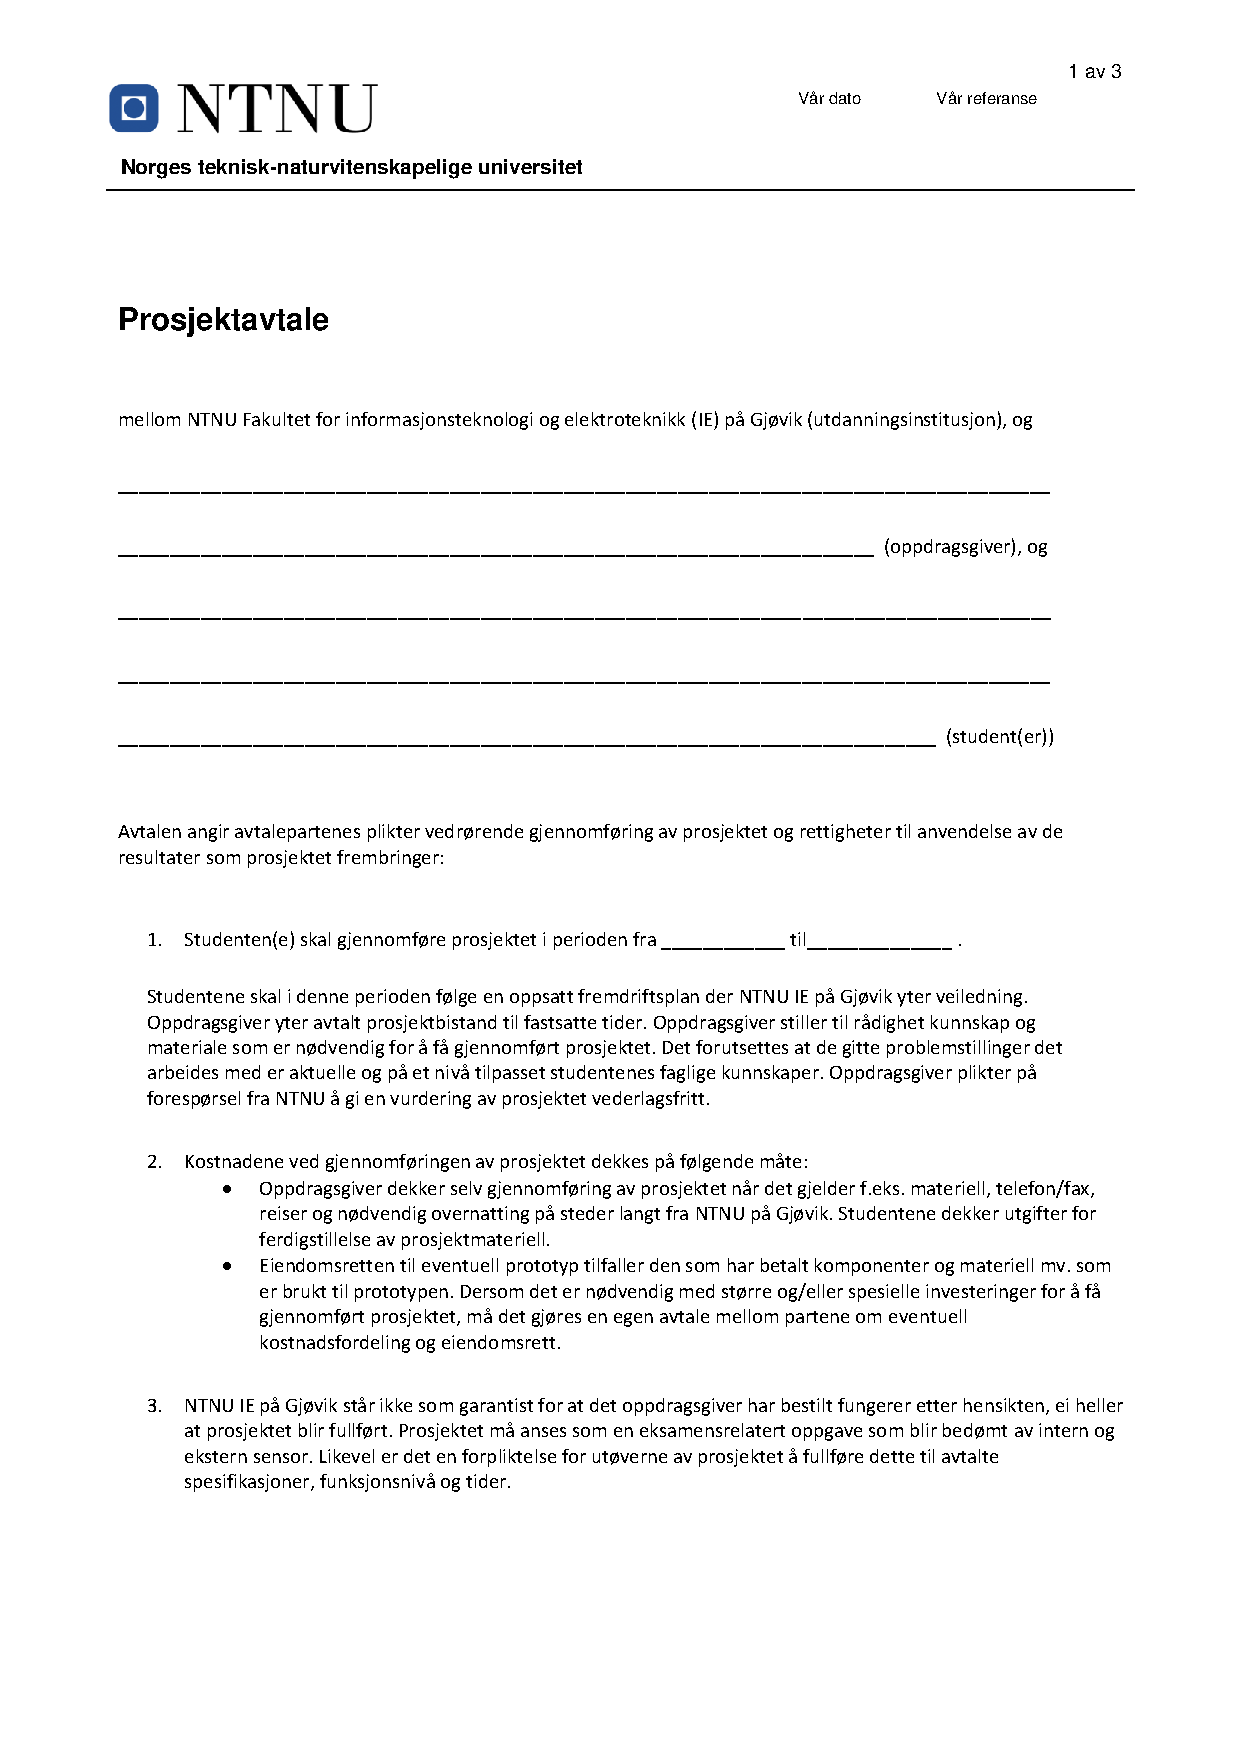
\includepdf[pages=-]{appendices/NTNUProsjektavtale.pdf}

\end{document}
